%%%%%%%%%%%%%%%%%%%%%%%%%%%%%%%%%%%%%%%%%%%%%%%%%%%%%%%%%%%%%%%%%%%%%%%%

%%% LaTeX Template for AAMAS-2025 (based on sample-sigconf.tex)
%%% Prepared by the AAMAS-2025 Program Chairs based on the version from AAMAS-2025. 

%%%%%%%%%%%%%%%%%%%%%%%%%%%%%%%%%%%%%%%%%%%%%%%%%%%%%%%%%%%%%%%%%%%%%%%%

%%% Start your document with the \documentclass command.


%%% == IMPORTANT ==
%%% Use the first variant below for the final paper (including auithor information).
%%% Use the second variant below to anonymize your submission (no authoir information shown).
%%% For further information on anonymity and double-blind reviewing, 
%%% please consult the call for paper information
%%% https://aamas2025.org/index.php/conference/calls/submission-instructions-main-technical-track/

\RequirePackage[2020-02-02]{latexrelease}

%%%% For anonymized submission, use this
\documentclass[sigconf,anonymous]{aamas} 

%%%% For camera-ready, use this
%\documentclass[sigconf]{aamas}

\usepackage{listings}
% \usepackage{xcolor}

\definecolor{codegreen}{rgb}{0,0.6,0}
\definecolor{codegray}{rgb}{0.5,0.5,0.5}
\definecolor{codepurple}{rgb}{0.58,0,0.82}
\definecolor{backcolour}{rgb}{0.95,0.95,0.92}
 
\lstdefinestyle{mystyle}{
    backgroundcolor=\color{backcolour},   
    commentstyle=\color{codegreen},
    keywordstyle=\color{magenta},
    numberstyle=\tiny\color{codegray},
    stringstyle=\color{codepurple},
    basicstyle=\footnotesize,
    breakatwhitespace=false,         
    breaklines=true,                 
    captionpos=b,                    
    keepspaces=true,                 
    numbers=left,                    
    numbersep=5pt,                  
    showspaces=false,                
    showstringspaces=false,
    showtabs=false,                  
    tabsize=2
}
 
\lstset{style=mystyle}

% --- Tickz
\usepackage{physics}
\usepackage{tikz}
\usepackage{amsmath}
\usepackage{mathdots}
% \usepackage{yhmath}
\usepackage{cancel}
\usepackage{color}
\usepackage{siunitx}
\usepackage{array}
\usepackage{multirow}
% \usepackage{amssymb}
\usepackage{gensymb}
\usepackage{tabularx}
\usepackage{extarrows}
\usepackage{booktabs}
\usetikzlibrary{fadings}
\usetikzlibrary{patterns}
\usetikzlibrary{shadows.blur}
\usetikzlibrary{shapes}

% ---------

\usepackage{balance} % for balancing columns on the final page
\usepackage{csquotes}
% \usepackage{cite}
\newcommand{\probP}{\text{I\kern-0.15em P}}
\usepackage{etoolbox}
\patchcmd{\thebibliography}{\section*{\refname}}{}{}{}
% \usepackage{amsthm,amssymb,amsfonts}

\usepackage[T1]{fontenc}
\usepackage{graphicx}
\usepackage{hyperref}
\usepackage{color}
% \renewcommand\UrlFont{\color{blue}\rmfamily}

\usepackage[inline, shortlabels]{enumitem}
\usepackage{tabularx}
\usepackage{caption}
\usepackage{listings}
\usepackage{titlesec}
\usepackage{ragged2e}
% \usepackage[hyphens]{url}
\usepackage[linesnumbered,ruled,vlined]{algorithm2e}
\usepackage{float}

\usepackage[english]{babel}
\addto\extrasenglish{  
    \def\figureautorefname{Figure}
    \def\tableautorefname{Table}
    \def\algorithmautorefname{Algorithm}
    \def\sectionautorefname{Section}
    \def\subsectionautorefname{Subsection}
    \def\proofoutlineautorefname{Proof Outline}
}

\newcommand{\supertiny}{\fontsize{1}{2}\selectfont}


%%%%%%%%%%%%%%%%%%%%%%%%%%%%%%%%%%%%%%%%%%%%%%%%%%%%%%%%%%%%%%%%%%%%%%%%

%%% AAMAS-2025 copyright block (do not change!)

\setcopyright{ifaamas}
\acmConference[AAMAS '25]{Proc.\@ of the 24th International Conference
on Autonomous Agents and Multiagent Systems (AAMAS 2025)}{May 19 -- 23, 2025}
{Detroit, Michigan, USA}{A.~El~Fallah~Seghrouchni, Y.~Vorobeychik, S.~Das, A.~Nowe (eds.)}
\copyrightyear{2025}
\acmYear{2025}
\acmDOI{}
\acmPrice{}
\acmISBN{}


%%%%%%%%%%%%%%%%%%%%%%%%%%%%%%%%%%%%%%%%%%%%%%%%%%%%%%%%%%%%%%%%%%%%%%%%

%%% == IMPORTANT ==
%%% Use this command to specify your EasyChair submission number.
%%% In anonymous mode, it will be printed on the first page.

\acmSubmissionID{<<EasyChair submission id>>}

%%% Use this command to specify the title of your paper.

\title[AAMAS-2025 CybMASDE]{Leveraging Organizations in MARL for Designing Multi-Agent Systems}

%%% Provide names, affiliations, and email addresses for all authors.

\author{Julien Soulé}
\affiliation{
  \institution{Univ. Grenoble Alpes}
  \city{Valence}
  \country{France}}
\email{julien.soule@lcis.grenoble-inp.fr}

\author{Jean-Paul Jamont}
\affiliation{
  \institution{Univ. Grenoble Alpes}
  \city{Valence}
  \country{France}}
\email{jean-paul.jamont@lcis.grenoble-inp.fr}

\author{Michel Occello}
\affiliation{
  \institution{Univ. Grenoble Alpes}
  \city{Valence}
  \country{France}}
\email{michel.occello@lcis.grenoble-inp.fr}

\author{Louis-Marie Traonouez}
\affiliation{
  \institution{Thales Land and Air Systems, BU IAS}
  \city{Rennes}
  \country{France}}
\email{louis-marie.traonouez@thalesgroup.com}

\author{Paul Théron}
\affiliation{
  \institution{AICA IWG}
  \city{La Guillermie}
  \country{France}}
\email{paul.theron@orange.fr}

\begin{abstract}
  Designing a Multi-Agent System to achieve a goal in an environment often requires an organizational structure to coordinate and delegate tasks among agents. However, defining the agents' internal logic can be challenging in complex environments. Multi-Agent Reinforcement Learning enables agents to learn how to reach a goal without explicitly considering the organization. While previous studies have introduced guided training in individual agents, a multi-agent context requires clarifying the implicit cooperation among multiple agents after training. We propose a novel algorithmic approach leveraging the $\mathcal{M}OISE^+$ Organizational Model that consists in linking organizational specifications, such as roles or missions, to the respective agents' histories, characterizing their behaviors. Our algorithm constrains the learning process based on organizational constraints. Evaluations conducted in a mixed competitive/cooperative Predator-Prey environment validate the impact of organizational specifications as constraints during training.
\end{abstract}

%%% The code below was generated by the tool at http://dl.acm.org/ccs.cfm.
%%% Please replace this example with code appropriate for your own paper.


%%% Use this command to specify a few keywords describing your work.
%%% Keywords should be separated by commas.

\keywords{Agent-Oriented Software Engineering \and Multi-Agent Reinforcement Learning \and Assisted-Design \and Organizational Models}

%%%%%%%%%%%%%%%%%%%%%%%%%%%%%%%%%%%%%%%%%%%%%%%%%%%%%%%%%%%%%%%%%%%%%%%%

%%% Include any author-defined commands here.
         
% \newcommand{\BibTeX}{\rm B\kern-.05em{\sc i\kern-.025em b}\kern-.08em\TeX}

%%%%%%%%%%%%%%%%%%%%%%%%%%%%%%%%%%%%%%%%%%%%%%%%%%%%%%%%%%%%%%%%%%%%%%%%

\begin{document}

%%% The following commands remove the headers in your paper. For final 
%%% papers, these will be inserted during the pagination process.

\pagestyle{fancy}
\fancyhead{}

%%% The next command prints the information defined in the preamble.

\maketitle

%%%%%%%%%%%%%%%%%%%%%%%%%%%%%%%%%%%%%%%%%%%%%%%%%%%%%%%%%%%%%%%%%%%%%%%%



\section{Introduction}
Multi-Agent Reinforcement Learning (MARL) has emerged as a powerful tool for developing intelligent agents capable of learning optimal behaviors through interactions with their environment. However, one of the key challenges in MARL is the lack of structured guidance during the learning process, which can lead to suboptimal policies, slow convergence, and unsafe behaviors. This is particularly problematic in real-world applications, such as autonomous driving and robotic coordination, where safety and stability are crucial.

In this paper, we address these challenges by integrating organizational models, specifically the MOISE+ framework, with MARL to provide structured guidance for agents during the learning process. By leveraging roles and missions defined in MOISE+, we constrain the policy space, enabling agents to focus on coordinated and safe behaviors while still exploring optimal strategies. Our approach, PRAHOMT, builds on the existing PRAHOM framework by explicitly linking agents' policies to organizational specifications, thus enhancing both explainability and stability.

The main contributions of this paper are as follows:
1. We introduce the PRAHOMT algorithm, which extends the PRAHOM approach by incorporating MOISE+ roles and missions into the learning process. This results in more structured and explainable agent behaviors.
2. We provide a comprehensive comparison of MOISE+ with other organizational models, such as AGR and S-MOISE+, and demonstrate the unique advantages of MOISE+ in the context of MARL.
3. We conduct extensive experiments in both simple and complex scenarios to evaluate the effectiveness of PRAHOMT. Our results show that PRAHOMT outperforms traditional MARL approaches and other optimization methods in terms of policy convergence, safety, and stability.

The rest of the paper is organized as follows. In Section 2, we discuss related works and position our approach within the existing literature. Section 3 presents the methodology, detailing the PRAHOMT algorithm and its integration with MOISE+. In Section 4, we present our experimental setup and results, followed by a discussion in Section 5. Finally, we conclude the paper in Section 6 and outline directions for future work.


\nocite{Kott2023}

% Context
In a top-down design approach, designing a Multi-Agent System (MAS) requires establishing an organization embeddable into the agents' internal logic (referred to as \textbf{policies}) that explains how agents coordinate their activities to collaboratively achieve a common expected goal~\cite{Picard2009}.
%
Consequently, designing a MAS can be viewed as an optimization problem, aiming to find the organization that promotes the best performance in achieving a goal. Methods such as GAIA~\cite{Wooldridge2000,Cernuzzi2014}, ADELFE~\cite{Mefteh2015}, or KB-ORG~\cite{Sims2008} rely on an iterative process of trial and error to gain knowledge of the environment and find an appropriate organization~\cite{Sims2008}.

% Problem
However, increasing this empirical knowledge can be costly for numerous factors including the environment's complexity or its restricted access, and the designers' unavailability. Moreover, relying solely on limited knowledge may prevent the designing of a MAS that meets sufficient performance or that guarantees safety requirements~\cite{Mefteh2013}. Currently, no method fully automate the design process of MAS. Meeting this challenge would improve the trust and adoption of MAS in real-world applications~\cite{kok2006collaborative,omidshafiei2019learning}.

% Contribution
To address this concern, we propose extending \textit{Partial Relation between Agents' History and Organizational Model}~\cite{soule2024} (PRAHOM). PRAHOM is a general approach that leverages histories to integrate $\mathcal{M}OISE^+$~\cite{Hubner2007} organizational model into the Multi-Agent Reinforcement Learning (MARL) framework. $\mathcal{M}OISE^+$ is suitable to represent organizational specifications in the MARL framework. It makes it possible to envision constraining the learning. However, the current development in this area remains limited and does not scale with the increasing number of organizational specifications. It is unsuitable for further application in more realistic scenarios.

Partially relying on PRAHOM, we propose a novel algorithm called \textit{PRAHOM Training} (PRAHOMT), which only requires the concepts of role and mission, thus addressing scalability issues.
% PRAHOMT can be seen as a way to assist MAS design.
PRAHOMT links $\mathcal{M}OISE^+$ and MARL by one-to-one mapping an organizational specification (i.e a role or a mission) to a history subset characterizing an expected behavior impacting action space or the reward function accordingly.
%
\autoref{fig:policy_histories} illustrates this underlying idea: a policy can be represented as the set of all its possibly generated histories/trajectories (arrows) in an abstract space representing all couples of joint-observations ($\Omega_{joint}$) and joint-actions ($A_{joint}$). A history starts from an initial observation-action couple (blue area) and possibly reaches one of the expected observation-action couples that characterize the goal (red area). The idea is to see a history subset as a way to characterize an organizational specification (orange area).

\begin{figure}[h!]
  \centering
  


\tikzset{every picture/.style={line width=0.75pt}} %set default line width to 0.75pt        

\begin{tikzpicture}[x=0.75pt,y=0.75pt,yscale=-1,xscale=1]
%uncomment if require: \path (0,839); %set diagram left start at 0, and has height of 839

%Shape: Rectangle [id:dp1150110825870514] 
\draw  [fill={rgb, 255:red, 255; green, 255; blue, 255 }  ,fill opacity=1 ] (80,225.71) -- (450,225.71) -- (450,424.53) -- (80,424.53) -- cycle ;
%Straight Lines [id:da7972096566562834] 
\draw [color={rgb, 255:red, 208; green, 2; blue, 27 }  ,draw opacity=1 ]   (367.35,251.8) -- (318.6,268.58) -- (228.54,303.1) -- (280.65,330.21) -- (243.79,323.82) -- (226.88,327.64) -- (226.88,350.23) -- (215.86,357.88) -- (213.85,359.27) -- (207.6,354.93) -- (187.8,341.2) -- (148.71,341.2) -- (154.93,345.51) -- (135.68,350.23) -- (142.4,359.55) -- (109.63,386.38) ;
\draw [shift={(370.19,250.82)}, rotate = 161.01] [fill={rgb, 255:red, 208; green, 2; blue, 27 }  ,fill opacity=1 ][line width=0.08]  [draw opacity=0] (3.57,-1.72) -- (0,0) -- (3.57,1.72) -- cycle    ;
%Straight Lines [id:da43171188229542157] 
\draw [color={rgb, 255:red, 80; green, 227; blue, 194 }  ,draw opacity=1 ]   (368.11,243.95) -- (344.14,268.9) -- (292.02,268.9) -- (292.02,286.97) -- (226.88,305.05) -- (239.91,314.09) -- (252.94,332.16) -- (213.85,323.12) -- (226.88,341.2) -- (213.85,341.2) -- (226.88,359.27) -- (200.83,359.27) -- (181.54,341.38) -- (174.77,354.75) -- (122.66,327.64) -- (161.74,359.27) -- (122.66,341.2) -- (135.68,359.27) -- (122.66,395.42) ;
\draw [shift={(370.19,241.79)}, rotate = 133.86] [fill={rgb, 255:red, 80; green, 227; blue, 194 }  ,fill opacity=1 ][line width=0.08]  [draw opacity=0] (3.57,-1.72) -- (0,0) -- (3.57,1.72) -- cycle    ;
%Straight Lines [id:da6941784709428771] 
\draw [color={rgb, 255:red, 248; green, 231; blue, 28 }  ,draw opacity=1 ]   (393.27,260.25) -- (324.79,269.18) -- (318.08,277.94) -- (272.68,287.25) -- (239.91,305.05) -- (243.79,323.82) -- (233.6,332.44) -- (213.85,314.09) -- (239.91,350.23) -- (239.91,359.27) -- (213.85,359.27) -- (162.2,341.66) -- (155.43,355.03) -- (116.34,359.55) -- (103.31,395.7) ;
\draw [shift={(396.25,259.86)}, rotate = 172.57] [fill={rgb, 255:red, 248; green, 231; blue, 28 }  ,fill opacity=1 ][line width=0.08]  [draw opacity=0] (3.57,-1.72) -- (0,0) -- (3.57,1.72) -- cycle    ;
%Straight Lines [id:da9725445694234951] 
\draw [color={rgb, 255:red, 144; green, 19; blue, 254 }  ,draw opacity=1 ]   (401.81,267.6) -- (419.7,270.71) -- (409.28,259.86) -- (398.85,252.63) -- (417.32,259.86) -- (430.12,270.71) -- (409.28,281.55) -- (422.3,296.01) -- (409.28,314.09) -- (422.3,323.12) -- (409.28,350.23) -- (409.28,386.38) -- (370.19,377.35) -- (344.14,377.35) -- (330.04,374.09) -- (322.58,372.36) -- (312,369.92) -- (305.05,368.31) -- (278.9,366.29) -- (258.15,364.69) -- (247.92,362.92) -- (226.88,359.27) -- (200.83,359.27) -- (187.8,368.31) -- (161.74,377.35) -- (161.74,395.42) ;
\draw [shift={(398.85,267.09)}, rotate = 9.84] [fill={rgb, 255:red, 144; green, 19; blue, 254 }  ,fill opacity=1 ][line width=0.08]  [draw opacity=0] (3.57,-1.72) -- (0,0) -- (3.57,1.72) -- cycle    ;
%Straight Lines [id:da8841659627316263] 
\draw [color={rgb, 255:red, 65; green, 117; blue, 5 }  ,draw opacity=1 ]   (399.2,269.41) -- (417.09,272.51) -- (406.67,261.67) -- (396.25,254.44) -- (414.71,261.67) -- (427.52,272.51) -- (409.28,292.4) -- (419.7,297.82) -- (414.49,324.93) -- (383.22,314.09) -- (409.28,328.54) -- (440.54,357.46) -- (398.85,335.77) -- (406.67,352.04) -- (414.49,379.15) -- (388.43,386.38) -- (346.74,371.92) -- (315.47,371.92) -- (299.84,371.92) -- (284.21,368.31) -- (278.99,375.54) -- (268.57,368.31) -- (273.78,379.15) -- (245.32,364.73) -- (224.28,361.08) -- (198.22,361.08) -- (185.19,370.12) -- (159.14,379.15) -- (159.14,397.23) ;
\draw [shift={(396.25,268.9)}, rotate = 9.84] [fill={rgb, 255:red, 65; green, 117; blue, 5 }  ,fill opacity=1 ][line width=0.08]  [draw opacity=0] (3.57,-1.72) -- (0,0) -- (3.57,1.72) -- cycle    ;
%Shape: Polygon Curved [id:ds6925092543976428] 
\draw  [color={rgb, 255:red, 74; green, 144; blue, 226 }  ,draw opacity=1 ][fill={rgb, 255:red, 74; green, 144; blue, 226 }  ,fill opacity=0.5 ] (90.53,390) .. controls (104.08,369.67) and (104.09,389.48) .. (120.23,390) .. controls (136.38,390.52) and (143.53,387.47) .. (149.94,390) .. controls (156.35,392.53) and (183.81,385.93) .. (181.73,399.04) .. controls (179.64,412.14) and (169.15,403.08) .. (149.09,400.82) .. controls (129.02,398.56) and (76.98,410.33) .. (90.53,390) -- cycle ;
%Shape: Polygon Curved [id:ds923152774229371] 
\draw  [color={rgb, 255:red, 208; green, 2; blue, 27 }  ,draw opacity=1 ][fill={rgb, 255:red, 208; green, 2; blue, 27 }  ,fill opacity=0.5 ] (357.16,250.82) .. controls (370.71,230.49) and (377.41,231.77) .. (370.19,241.79) .. controls (362.97,251.8) and (393.64,237.04) .. (391.56,250.15) .. controls (389.47,263.25) and (429.34,271.16) .. (409.28,268.9) .. controls (389.21,266.64) and (343.61,271.16) .. (357.16,250.82) -- cycle ;
%Shape: Ellipse [id:dp804778882822857] 
\draw  [color={rgb, 255:red, 74; green, 144; blue, 226 }  ,draw opacity=1 ][fill={rgb, 255:red, 80; green, 227; blue, 194 }  ,fill opacity=1 ] (360,445) .. controls (360,442.24) and (364.48,440) .. (370,440) .. controls (375.52,440) and (380,442.24) .. (380,445) .. controls (380,447.76) and (375.52,450) .. (370,450) .. controls (364.48,450) and (360,447.76) .. (360,445) -- cycle ;
%Straight Lines [id:da8876833624261078] 
\draw [color={rgb, 255:red, 0; green, 0; blue, 0 }  ,draw opacity=1 ]   (197.88,442.12) -- (190,450) -- (190,440) -- (180,450) ;
\draw [shift={(200,440)}, rotate = 135] [fill={rgb, 255:red, 0; green, 0; blue, 0 }  ,fill opacity=1 ][line width=0.08]  [draw opacity=0] (3.57,-1.72) -- (0,0) -- (3.57,1.72) -- cycle    ;
%Straight Lines [id:da7575795561031657] 
\draw    (135.09,390) -- (105.38,350) -- (164.79,350) -- (120.23,320) -- (164.79,330) -- (150.98,292.81) ;
\draw [shift={(149.94,290)}, rotate = 69.63] [fill={rgb, 255:red, 0; green, 0; blue, 0 }  ][line width=0.08]  [draw opacity=0] (3.57,-1.72) -- (0,0) -- (3.57,1.72) -- cycle    ;
%Straight Lines [id:da04182102181099867] 
\draw [color={rgb, 255:red, 155; green, 155; blue, 155 }  ,draw opacity=1 ]   (179.65,400) -- (209.35,380) -- (253.91,390) -- (298.47,390) -- (313.32,400) -- (369.73,400) ;
\draw [shift={(372.73,400)}, rotate = 180] [fill={rgb, 255:red, 155; green, 155; blue, 155 }  ,fill opacity=1 ][line width=0.08]  [draw opacity=0] (3.57,-1.72) -- (0,0) -- (3.57,1.72) -- cycle    ;
%Shape: Polygon [id:ds12618969894880627] 
\draw  [color={rgb, 255:red, 255; green, 255; blue, 255 }  ,draw opacity=1 ][fill={rgb, 255:red, 245; green, 166; blue, 35 }  ,fill opacity=0.37 ][dash pattern={on 4.5pt off 4.5pt}] (432.14,260) -- (447,360) -- (417.29,360) -- (415.6,388.61) -- (328.17,380) -- (268.76,380) -- (194.5,370) -- (164.79,380) -- (164.79,400) -- (149.94,390) -- (164.79,370) -- (179.65,370) -- (200.83,359.27) -- (239.06,360) -- (346.74,371.92) -- (387.59,380) -- (402.44,370) -- (387.59,330) -- (402.44,330) -- (402.44,320) -- (402.44,280) -- (391.56,250.15) -- cycle ;
%Shape: Ellipse [id:dp19993377935309375] 
\draw  [color={rgb, 255:red, 255; green, 255; blue, 255 }  ,draw opacity=1 ][fill={rgb, 255:red, 245; green, 166; blue, 35 }  ,fill opacity=0.57 ] (40,445) .. controls (40,442.24) and (44.48,440) .. (50,440) .. controls (55.52,440) and (60,442.24) .. (60,445) .. controls (60,447.76) and (55.52,450) .. (50,450) .. controls (44.48,450) and (40,447.76) .. (40,445) -- cycle ;


% Text Node
\draw (116,442.5) node  [font=\scriptsize,color={rgb, 255:red, 0; green, 0; blue, 0 }  ,opacity=1 ] [align=left] {Joint-History Subset};
% Text Node
\draw (274.5,445.5) node  [font=\scriptsize,color={rgb, 255:red, 0; green, 0; blue, 0 }  ,opacity=1 ] [align=left] {Joint-Observations-Actions\\Trajectory/History};
% Text Node
\draw (438,445.5) node  [font=\scriptsize,color={rgb, 255:red, 0; green, 0; blue, 0 }  ,opacity=1 ] [align=left] {Joint-Observations\\\mbox{-}Actions Subset};
% Text Node
\draw (308.69,235.75) node  [font=\tiny,color={rgb, 255:red, 208; green, 2; blue, 27 }  ,opacity=1 ] [align=left] {$\displaystyle \Omega _{joint,goal} \times A_{joint,goal}$};
% Text Node
\draw (145.27,249.45) node  [font=\small,color={rgb, 255:red, 0; green, 0; blue, 0 }  ,opacity=1 ] [align=left] {$\displaystyle \Omega _{joint} \times A_{joint}$};
% Text Node
\draw (240.34,410.27) node  [font=\tiny,color={rgb, 255:red, 74; green, 144; blue, 226 }  ,opacity=1 ] [align=left] {$\displaystyle \Omega _{joint,init} \times A_{joint,init}$};


\end{tikzpicture}
  \caption{An abstract view of joint-policy as joint-histories and constraints}
  \label{fig:policy_histories}
\end{figure}

Unlike, classical MARL where an agent's policy is freely updated solely based on maximizing the reward, our approach also forces/entices agents to satisfy some hand-crafted organizational specifications during the training. By restricting the policy search space, our approach may shorten the convergence time. It enables stabilizing resulting policies during/after training. From a design point of view, the obtained policies can be analyzed as fine-tuned organizations leveraging known introduced organizational specifications to help out with explainability. This led to getting relevant insights into future design in the real environment. Although adding organizational specifications may also prevent new organizations from emerging, our contribution provides practical means for users to find a tradeoff while addressing safety guarantees.

% Outline
The remainder is organized as follows: \autoref{sec:marl_background} presents the MARL framework our contribution is built on. \autoref{sec:related_works} gives an overview of the available works dealing with modifying policies within MARL. \autoref{sec:linking_marl_moise} presents the proposed principles to link $\mathcal{M}OISE^+$ and MARL. \autoref{sec:prahom_alg} introduces the PRAHOMT algorithm. \autoref{sec:case_study} first presents our PRAHOMT implementation as a library we used in our experimental setup, and discusses the results of our evaluation. \autoref{sec:conclusion} concludes the paper and outlines future research directions.


\section{MARL background}\label{sec:marl_background}

MARL extends the concepts of Reinforcement Learning (RL) to multi-agent context. Agents' policies are optimized to maximize the total cumulative reward through learning.
To apply MARL techniques, we chose the Decentralized Partially Observable Markov Decision Process (Dec-POMDP)~\cite{Oliehoek2016} because it considers multiple agents in a similar MAS manner. It relies on stochastic processes to model the uncertainty of the environment for the changes induced by actions, received observations, and communication. Additionally, unlike Partially Observable Stochastic Games, the reward function can be common to agents which fosters training for collaborative-oriented actions~\cite{Beynier2013}.

A Dec-POMDP $d \in D$ (with $D$ the set of Dec-POMDP) is a 7-tuple $d = (S,\{A_i\},T,R,\{\Omega_i\},O,\gamma)$ , where:
$S = \{s_1,\dots,s_{|S|}\}$: the set of possible states;
$A_{i} = \{a_{1}^{i},\dots,a_{|A_{i}|}^{i}\}$: the set of possible actions for agent $i$;
$T$ so that $T(s,a,s') = \probP{(s'|s,a)}$ : the set of conditional transition probabilities between states;
$R: S \times A \times S \rightarrow \mathbb{R}$: the reward function;
$\Omega_{i} = \{o_{1}^{i},\dots,o_{|\Omega_{i}|}^{i}\}$: the set of observations for agent $i$;
$O$ so that $O(s',a,o) = \probP{(o|s',a)}$ : the set of conditional observation probabilities;
$\gamma \in [0,1]$ : the discount factor.

Considering $m$ \textbf{teams} (also referred to as \textbf{groups}) each containing several agents among $\mathcal{A}$, we also detail the minimal formalism notation we re-used for solving the Dec-POMDP for a given team $i, 0 \leq i \leq m$ containing $n$ agents~\cite{Beynier2013,Albrecht2024}:

\begin{itemize}

  \item $\Pi$: the set of policies. A \textbf{policy} $\pi \in \Pi, \pi: H \times \Omega \rightarrow A$ associates an observation to an action optionally using previous experiences as histories. It represents the agent's internal logic;
  \item $\Pi_{joint}$: the set of joint-policies. A \textbf{joint-policy} $\pi_{joint} \in \Pi_{joint}, \pi_{joint}: H_{joint} \times \Omega^n \rightarrow A^n = \Pi^n$ chooses an action for each agent regarding their respective observation optionally using previous experiences as histories. It can be viewed as a set of policies used in agents;
  \item $H$: the set of histories. A \textbf{history} over $z \in \mathbb{N}$ steps (where $z$ is generally the maximum number of steps for an episode) is the $z$-tuple $h = ((\omega_{k}, a_{k}) | k \leq z, \omega \in \Omega, a \in A)$;
  \item $H_{joint}$: the set of joint-histories. A \textbf{joint-history} over $z \in \mathbb{N}$ steps $h_{joint} \in H_{joint}, h_{joint} = \{h_1,h_2 \dots h_n\}$ is the set of agents' histories;
  \item $U_{joint,i}(<\pi_{joint,i}, \pi_{joint,-i}>): \Pi_{joint} \rightarrow \mathbb{R}$: gives the \textbf{expected cumulative reward} over a finite horizon (if $\gamma < 1$ or the number of steps in an episode is finite), with $\pi_{joint,i}$ the joint policy for team $i$ and $\pi_{joint,-i}$ all of the other concatenated joint-policies (considered as fixed).
        % \item $BR_{joint,i}(\pi_{joint,i}) = argmax_{\pi_{joint,i}}(U(<\pi_{joint,i},\pi_{joint,-i}>))$: gives the \textbf{best response} $\pi_{joint,i}^*$ in the sense that the team cannot change any of the policies in the joint-policy $\pi_{joint,i}^*$ to get a better expected cumulative reward than $U_i^* = U_{joint,i}(<\pi_{joint,i}^*, \pi_{joint,-i}>)$;
        % \item $SR_{joint,i}(\pi_{joint,i}, s) = \{\pi_{joint,i} | U(<\pi_{joint,i},\pi_{joint,-i}>) \geq s\}$: gives the \textbf{sufficient response} as the set of joint-policies getting at least $s \in \mathbb{R}, s \leq U_i^*$ as expected cumulative reward.
\end{itemize}

Various approaches enable solving MARL problems. We favored \textbf{Policy-based} methods, such as Multi-Agent Proximal Policy Optimization~\cite{yu2022surprising} (MAPPO) and Multi-Agent Deep Deterministic Policy Gradient~\cite{Lowe2017}. These algorithms directly parameterize the policy as $\pi_\theta$ to optimize it possibly using Centralized Learning and Decentralized Execution.
We refer to \textbf{solving} the Dec-POMDP at $s$ expectancy as finding the joint policies $\pi_{joint,i} \in \Pi_{joint}, \pi_{joint,i} = \{\pi_{joint,i} | U(<\pi_{joint,i},\pi_{joint,-i}>) \geq s\}$ that gets the expected cumulative reward over a finite horizon at least at $s \in \mathbb{R}$.


\section{Related works and positioning}\label{sec:related_works}

The integration of organizational specifications in MAS learning processes is not largely addressed explicitly in the literature. Yet, various approaches have been proposed to incorporate organizational constraints and policies in MAS to ensure agents adhere to certain requirements.

\textbf{Learning with Organizational Constraints} \quad
%
The integration of organizational constraints into the learning process of agents has been explored to various extents. In \cite{cruz2020norms}, the authors present a method for incorporating norms into the learning algorithms of agents, ensuring that their behavior remains within acceptable bounds. Additionally, \cite{villatoro2011social} proposes a mechanism for agents to learn and adapt to social norms in dynamic environments, highlighting the importance of norm adaptation in MAS. However, these norms cannot be individual.

\emph{Specification-Guided Reinforcement Learning} aims to generate policies that accomplish a specific task using external specifications to guide learning in achieving an objective under given constraints~\cite{Bansal2022}. Jothimurugan et al.~\cite{Jothimurugan2021} propose logical specification learning as exploiting the compositional structure of specifications to generate policies for complex tasks. However, it does not completely fall into the MARL framework we set for it requires introducing logical specifications.

\textbf{Policy-Based Approaches} \quad
%
Policy-based approaches provide a way to enforce organizational constraints by defining explicit policies that govern agent behavior. In \cite{krupanski2015norm}, the use of normative policies is investigated to guide agent interactions and decision-making processes. Moreover, \cite{vos2020governing} explores the use of governance mechanisms to enforce compliance with organizational policies in decentralized systems. However, these approaches face a lack of explainability since most policies are black-box and cannot be easily modified.

\textbf{Frameworks Integrating Organizational Aspects} \quad
%
Wang et al.~\cite{Wang2020} introduce an approach in which similar emerging roles are pushed to jointly specialize in specific tasks. Tosic et al.~\cite{Tosic2010} propose a framework for coordination based on the communication capabilities of multi-agent systems. Zheng et al.~\cite{Zheng2018} present a platform for MARL that aims to facilitate research on artificial collective intelligence by providing a comprehensive set of evaluation metrics to compare the performance of MARL algorithms. However, it does not take into account specifications likely to entice agents to adhere to an expected behavior such as missions.

\

Despite these advancements, there is still a lack of works that explicitly use organizational specifications as a means of constraining agent learning regarding requirements. To our knowledge, no work can be used to generate a MAS that satisfies additional organizational constraints explicitly. Unlike these works, our originality is to explicitly use an organizational model as a general means of constraining learning regarding requirements.


\section{Linking MARL and the $\mathcal{M}OISE^+$ model}\label{sec:linking_marl_moise}
\label{sec:marl_moise_linking}

In this section, we incrementally present the principles we propose to adapt the MARL according to organizational specifications. This includes constraining a policy to adhere to the expected behavior of a role and enticing the policy to achieve a mission for a given time duration.


The $\mathcal{M}OISE^+$ model provides a comprehensive framework for specifying the structure and interactions within a Multi-Agent System (MAS). We utilize $\mathcal{M}OISE^+$ due to its compatibility with MARL and its formal description capabilities for agents' policies. The PRAHOMT's underlying approach bridges the gap between MARL and organizational modeling by embedding $\mathcal{M}OISE^+$ specifications into the MARL training process. This integration allows for the training of agents that adhere to predefined organizational roles and missions.
%
In $\mathcal{M}OISE^+$, \textbf{Organizational Specifications (OS)} are defined as $\mathcal{OS} = \langle \mathcal{SS}, \mathcal{FS}, \mathcal{DS} \rangle$, where $\mathcal{SS}$ are the \textbf{Structural Specifications}, $\mathcal{FS}$ are the \textbf{Functional Specifications}, and $\mathcal{DS}$ are the \textbf{Deontic Specifications}.

\subsection{Structural Specifications and Constraining Joint-Policies According to Roles}

\textbf{Structural Specifications} describe the organizational structure and are denoted as $\mathcal{SS} = \langle \mathcal{R}, \mathcal{IR}, \mathcal{G} \rangle$:

\begin{itemize}
  \item $\mathcal{R}_{ss}$: The set of all roles ($\rho \in \mathcal{R}$).
  \item $\mathcal{IR}: \mathcal{R} \rightarrow \mathcal{R}$: The inheritance relation between roles ($\rho_1 \sqsubset \rho_2$).
  \item $\mathcal{RG} \subseteq \mathcal{GR}$: The set of root groups, $\mathcal{GR} = \langle \mathcal{R}, \mathcal{SG}, \mathcal{L}^{intra}, \mathcal{L}^{inter}, \mathcal{C}^{intra}, \mathcal{C}^{inter}, \allowbreak np, ng \rangle$, where:
        %   \begin{itemize}
        $\mathcal{R} \subseteq \mathcal{R}_{ss}$: The set of non-abstract roles.
        $\mathcal{SG} \subseteq \mathcal{GR}$: The set of sub-groups.
        $\mathcal{L} = \mathcal{R} \times \mathcal{R} \times \mathcal{TL}$: The set of links $(\rho_s, \rho_d, t)$, where $t \in \{acq, com, aut\}$ indicates the type of link (acquaintance, communication, authority).
        $\mathcal{L}^{intra} \subseteq \mathcal{L}$: The set of intra-group links.
        $\mathcal{L}^{inter} \subseteq \mathcal{L}$: The set of inter-group links.
        $\mathcal{C} = \mathcal{R} \times \mathcal{R}$: The set of compatibilities $(\rho_a \bowtie \rho_b)$.
        $\mathcal{C}^{intra} \subseteq \mathcal{C}$: The set of intra-group compatibilities.
        $\mathcal{C}^{inter} \subseteq \mathcal{C}$: The set of inter-group compatibilities.
        $np: \mathcal{R} \rightarrow \mathbb{N} \times \mathbb{N}$: The cardinality of agents adopting a role.
        $ng: \mathcal{SG} \rightarrow \mathbb{N} \times \mathbb{N}$: The cardinality of each sub-group.
        %   \end{itemize}
\end{itemize}

Constraining policies directly is not feasible because most policy implementations rely on intractable black-box models such as neural networks. We propose to formally represent a role as a history subset $\mathcal{P}(H)$ containing histories an agent playing a role should generate, hence characterizing the role's expected behavior. As illustrated in \autoref{fig:PRAHOM_osm_rels}, we propose each role to be mapped to a history subset through the $rh: \mathcal{R} \rightarrow \mathcal{P}(H)$ bijection. An agent playing a role should have its policy constrained to generate histories belonging to the mapped history subset (at least from a theoretical point of view).

\begin{figure}[h!]
  \centering
  


\tikzset{every picture/.style={line width=0.75pt}} %set default line width to 0.75pt        

\begin{tikzpicture}[x=0.75pt,y=0.75pt,yscale=-1,xscale=1]
%uncomment if require: \path (0,1800); %set diagram left start at 0, and has height of 1800

%Shape: Rectangle [id:dp9341453924522656] 
\draw  [fill={rgb, 255:red, 255; green, 255; blue, 255 }  ,fill opacity=1 ] (160,44) -- (510,44) -- (510,167) -- (160,167) -- cycle ;
%Shape: Rectangle [id:dp4628140741854456] 
\draw  [fill={rgb, 255:red, 184; green, 233; blue, 134 }  ,fill opacity=0.34 ] (374,52) -- (504,52) -- (504,162) -- (374,162) -- cycle ;
%Shape: Rectangle [id:dp6461749357206974] 
\draw  [fill={rgb, 255:red, 184; green, 233; blue, 134 }  ,fill opacity=0.34 ] (378,78) -- (500,78) -- (500,158) -- (378,158) -- cycle ;
%Shape: Rectangle [id:dp47018118728898073] 
\draw  [fill={rgb, 255:red, 248; green, 231; blue, 28 }  ,fill opacity=0.4 ] (164,48) -- (314,48) -- (314,162) -- (164,162) -- cycle ;
%Straight Lines [id:da37904402438854] 
\draw    (400,150.31) -- (400,193.69) ;
\draw [shift={(400,195.69)}, rotate = 270] [color={rgb, 255:red, 0; green, 0; blue, 0 }  ][line width=0.75]    (10.93,-3.29) .. controls (6.95,-1.4) and (3.31,-0.3) .. (0,0) .. controls (3.31,0.3) and (6.95,1.4) .. (10.93,3.29)   ;
\draw [shift={(400,148.31)}, rotate = 90] [color={rgb, 255:red, 0; green, 0; blue, 0 }  ][line width=0.75]    (10.93,-3.29) .. controls (6.95,-1.4) and (3.31,-0.3) .. (0,0) .. controls (3.31,0.3) and (6.95,1.4) .. (10.93,3.29)   ;
%Straight Lines [id:da30557994145553513] 
\draw    (368,140) -- (386,140) ;
\draw [shift={(388,140)}, rotate = 180] [color={rgb, 255:red, 0; green, 0; blue, 0 }  ][line width=0.75]    (10.93,-3.29) .. controls (6.95,-1.4) and (3.31,-0.3) .. (0,0) .. controls (3.31,0.3) and (6.95,1.4) .. (10.93,3.29)   ;
%Shape: Rectangle [id:dp15689957472567295] 
\draw  [fill={rgb, 255:red, 248; green, 231; blue, 28 }  ,fill opacity=0.4 ] (169.56,76) -- (309.06,76) -- (309.06,157) -- (169.56,157) -- cycle ;
%Shape: Rectangle [id:dp6202366628126772] 
\draw  [fill={rgb, 255:red, 255; green, 255; blue, 255 }  ,fill opacity=1 ] (372,196) -- (414,196) -- (414,216) -- (372,216) -- cycle ;

%Shape: Rectangle [id:dp20067598884831228] 
\draw  [fill={rgb, 255:red, 248; green, 231; blue, 28 }  ,fill opacity=0.4 ] (212.06,129) -- (234.06,129) -- (234.06,149) -- (212.06,149) -- cycle ;

%Shape: Rectangle [id:dp5970765798398485] 
\draw  [fill={rgb, 255:red, 248; green, 231; blue, 28 }  ,fill opacity=0.4 ] (178.06,129) -- (203.06,129) -- (203.06,149) -- (178.06,149) -- cycle ;
%Shape: Rectangle [id:dp92237875722883] 
\draw  [fill={rgb, 255:red, 248; green, 231; blue, 28 }  ,fill opacity=0.4 ] (178.06,102) -- (218.06,102) -- (218.06,122) -- (178.06,122) -- cycle ;

%Shape: Rectangle [id:dp6591761395302378] 
\draw  [fill={rgb, 255:red, 248; green, 231; blue, 28 }  ,fill opacity=0.4 ] (178.06,80) -- (218.06,80) -- (218.06,100) -- (178.06,100) -- cycle ;

%Shape: Rectangle [id:dp11794703752595392] 
\draw  [fill={rgb, 255:red, 248; green, 231; blue, 28 }  ,fill opacity=0.4 ] (258.5,80) -- (298.5,80) -- (298.5,100) -- (258.5,100) -- cycle ;

%Shape: Rectangle [id:dp6557958558103134] 
\draw  [fill={rgb, 255:red, 248; green, 231; blue, 28 }  ,fill opacity=0.4 ] (259,102) -- (299,102) -- (299,122) -- (259,122) -- cycle ;

%Shape: Rectangle [id:dp8284992701408749] 
\draw  [fill={rgb, 255:red, 65; green, 117; blue, 5 }  ,fill opacity=1 ] (388,129) -- (410,129) -- (410,149) -- (388,149) -- cycle ;

%Shape: Rectangle [id:dp7066110016250453] 
\draw  [fill={rgb, 255:red, 248; green, 231; blue, 28 }  ,fill opacity=0.4 ] (244,129) -- (266,129) -- (266,149) -- (244,149) -- cycle ;

%Shape: Rectangle [id:dp4021333114319714] 
\draw  [fill={rgb, 255:red, 248; green, 231; blue, 28 }  ,fill opacity=0.4 ] (170.31,53) -- (195.69,53) -- (195.69,73) -- (170.31,73) -- cycle ;

%Shape: Rectangle [id:dp8476756388266236] 
\draw  [fill={rgb, 255:red, 248; green, 231; blue, 28 }  ,fill opacity=0.4 ] (200,53) -- (226,53) -- (226,73) -- (200,73) -- cycle ;

%Shape: Rectangle [id:dp07470576340681823] 
\draw  [fill={rgb, 255:red, 74; green, 144; blue, 226 }  ,fill opacity=1 ] (324,101) -- (364,101) -- (364,121) -- (324,121) -- cycle ;

%Shape: Rectangle [id:dp31407652093057714] 
\draw  [fill={rgb, 255:red, 74; green, 144; blue, 226 }  ,fill opacity=1 ] (324,129) -- (364,129) -- (364,149) -- (324,149) -- cycle ;

%Shape: Rectangle [id:dp053729126169398844] 
\draw  [fill={rgb, 255:red, 184; green, 233; blue, 134 }  ,fill opacity=0.34 ] (378,55) -- (404,55) -- (404,75) -- (378,75) -- cycle ;

%Shape: Rectangle [id:dp7720103442630182] 
\draw  [fill={rgb, 255:red, 184; green, 233; blue, 134 }  ,fill opacity=0.34 ] (405.94,103) -- (431.94,103) -- (431.94,123) -- (405.94,123) -- cycle ;

%Shape: Rectangle [id:dp3183552657000306] 
\draw  [fill={rgb, 255:red, 184; green, 233; blue, 134 }  ,fill opacity=0.34 ] (447.44,103) -- (473.44,103) -- (473.44,123) -- (447.44,123) -- cycle ;

%Shape: Rectangle [id:dp10802424702469593] 
\draw  [fill={rgb, 255:red, 184; green, 233; blue, 134 }  ,fill opacity=0.34 ] (466,129) -- (488,129) -- (488,149) -- (466,149) -- cycle ;

%Shape: Rectangle [id:dp16589412198505937] 
\draw  [fill={rgb, 255:red, 184; green, 233; blue, 134 }  ,fill opacity=0.34 ] (428,129) -- (450,129) -- (450,149) -- (428,149) -- cycle ;

%Shape: Rectangle [id:dp1270989692188249] 
\draw  [fill={rgb, 255:red, 255; green, 255; blue, 255 }  ,fill opacity=1 ] (258,196) -- (300,196) -- (300,216) -- (258,216) -- cycle ;

%Straight Lines [id:da40017392935840324] 
\draw    (286,149.69) -- (286,193.69) ;
\draw [shift={(286,195.69)}, rotate = 270] [color={rgb, 255:red, 0; green, 0; blue, 0 }  ][line width=0.75]    (10.93,-3.29) .. controls (6.95,-1.4) and (3.31,-0.3) .. (0,0) .. controls (3.31,0.3) and (6.95,1.4) .. (10.93,3.29)   ;
\draw [shift={(286,147.69)}, rotate = 90] [color={rgb, 255:red, 0; green, 0; blue, 0 }  ][line width=0.75]    (10.93,-3.29) .. controls (6.95,-1.4) and (3.31,-0.3) .. (0,0) .. controls (3.31,0.3) and (6.95,1.4) .. (10.93,3.29)   ;
%Shape: Rectangle [id:dp21027747628033966] 
\draw  [fill={rgb, 255:red, 245; green, 166; blue, 35 }  ,fill opacity=1 ] (276,129) -- (298,129) -- (298,149) -- (276,149) -- cycle ;

%Shape: Rectangle [id:dp5582162899072272] 
\draw  [fill={rgb, 255:red, 255; green, 255; blue, 255 }  ,fill opacity=1 ] (172,178) -- (184,178) -- (184,190) -- (172,190) -- cycle ;
%Straight Lines [id:da3472969066473863] 
\draw    (170,210) -- (192,210) ;
\draw [shift={(194,210)}, rotate = 180] [color={rgb, 255:red, 0; green, 0; blue, 0 }  ][line width=0.75]    (6.56,-1.97) .. controls (4.17,-0.84) and (1.99,-0.18) .. (0,0) .. controls (1.99,0.18) and (4.17,0.84) .. (6.56,1.97)   ;
\draw [shift={(168,210)}, rotate = 0] [color={rgb, 255:red, 0; green, 0; blue, 0 }  ][line width=0.75]    (6.56,-1.97) .. controls (4.17,-0.84) and (1.99,-0.18) .. (0,0) .. controls (1.99,0.18) and (4.17,0.84) .. (6.56,1.97)   ;
%Shape: Rectangle [id:dp07012270906311535] 
\draw  [fill={rgb, 255:red, 255; green, 255; blue, 255 }  ,fill opacity=1 ] (332,197) -- (354,197) -- (354,217) -- (332,217) -- cycle ;

%Straight Lines [id:da7534392810513293] 
\draw    (344,164) -- (344,194) ;
\draw [shift={(344,196)}, rotate = 270] [color={rgb, 255:red, 0; green, 0; blue, 0 }  ][line width=0.75]    (10.93,-3.29) .. controls (6.95,-1.4) and (3.31,-0.3) .. (0,0) .. controls (3.31,0.3) and (6.95,1.4) .. (10.93,3.29)   ;
\draw [shift={(344,162)}, rotate = 90] [color={rgb, 255:red, 0; green, 0; blue, 0 }  ][line width=0.75]    (10.93,-3.29) .. controls (6.95,-1.4) and (3.31,-0.3) .. (0,0) .. controls (3.31,0.3) and (6.95,1.4) .. (10.93,3.29)   ;
%Straight Lines [id:da4125176624573814] 
\draw    (320,140) -- (300,140) ;
\draw [shift={(298,140)}, rotate = 360] [color={rgb, 255:red, 0; green, 0; blue, 0 }  ][line width=0.75]    (10.93,-3.29) .. controls (6.95,-1.4) and (3.31,-0.3) .. (0,0) .. controls (3.31,0.3) and (6.95,1.4) .. (10.93,3.29)   ;
%Shape: Rectangle [id:dp005426842763594397] 
\draw  [fill={rgb, 255:red, 80; green, 227; blue, 194 }  ,fill opacity=0.36 ] (320,76) -- (368,76) -- (368,162) -- (320,162) -- cycle ;
%Straight Lines [id:da9128713017721406] 
\draw    (478,150.31) -- (478,193.69) ;
\draw [shift={(478,195.69)}, rotate = 270] [color={rgb, 255:red, 0; green, 0; blue, 0 }  ][line width=0.75]    (10.93,-3.29) .. controls (6.95,-1.4) and (3.31,-0.3) .. (0,0) .. controls (3.31,0.3) and (6.95,1.4) .. (10.93,3.29)   ;
\draw [shift={(478,148.31)}, rotate = 90] [color={rgb, 255:red, 0; green, 0; blue, 0 }  ][line width=0.75]    (10.93,-3.29) .. controls (6.95,-1.4) and (3.31,-0.3) .. (0,0) .. controls (3.31,0.3) and (6.95,1.4) .. (10.93,3.29)   ;
%Shape: Rectangle [id:dp7604827971406838] 
\draw  [fill={rgb, 255:red, 255; green, 255; blue, 255 }  ,fill opacity=1 ] (450,196) -- (492,196) -- (492,216) -- (450,216) -- cycle ;



% Text Node
\draw (465,179) node   [align=left] {$gh$};
% Text Node
\draw (181.5,204) node  [font=\tiny] [align=left] {$name$};
% Text Node
\draw (334,179) node   [align=left] {$da$};
% Text Node
\draw (222,207) node  [font=\footnotesize] [align=left] {\begin{minipage}[lt]{29.67pt}\setlength\topsep{0pt}
\begin{center}
{\small Relation}
\end{center}

\end{minipage}};
% Text Node
\draw (202,185) node  [font=\footnotesize] [align=left] {\begin{minipage}[lt]{13.75pt}\setlength\topsep{0pt}
\begin{center}
{\small Set}
\end{center}

\end{minipage}};
% Text Node
\draw (343.5,61) node   [align=left] {$\mathcal{OS}$};
% Text Node
\draw (190.56,139) node   [align=left] {$\mathcal{SG}$};
% Text Node
\draw (345,85) node   [align=left] {$\mathcal{DS}$};
% Text Node
\draw (245.5,61) node   [align=left] {$\mathcal{SS}$};
% Text Node
\draw (387,179) node   [align=left] {$mh$};
% Text Node
\draw (275.5,177) node   [align=left] {$rh$};
% Text Node
\draw (237.56,91) node   [align=left] {$\mathcal{G}r$};
% Text Node
\draw (440.5,65) node   [align=left] {$\mathcal{FS}$};
% Text Node
\draw (439.44,90) node   [align=left] {$\mathcal{SCH}$};
% Text Node
\draw (472,205) node   [align=left] {$\mathcal{P}(H)$};
% Text Node
\draw (343,207) node   [align=left] {$\mathcal{A}$};
% Text Node
\draw (287,139) node   [align=left] {$\mathcal{R}$};
% Text Node
\draw (280,205) node   [align=left] {$\mathcal{P}(H)$};
% Text Node
\draw (439,139) node   [align=left] {$\mathcal{P}$};
% Text Node
\draw (477,139) node   [align=left] {$\mathcal{G}$};
% Text Node
\draw (460.44,113) node   [align=left] {$nm$};
% Text Node
\draw (418.94,113) node   [align=left] {$mo$};
% Text Node
\draw (391,65) node   [align=left] {$\mathcal{PO}$};
% Text Node
\draw (345,139) node   [align=left] {$\mathcal{OBL}$};
% Text Node
\draw (345,111) node   [align=left] {$\mathcal{PER}$};
% Text Node
\draw (214,62) node   [align=left] {$\mathcal{R}_{ss}$};
% Text Node
\draw (183,63) node   [align=left] {$\mathcal{IR}$};
% Text Node
\draw (255,139) node   [align=left] {$\mathnormal{ng}$};
% Text Node
\draw (399,139) node   [align=left] {$\mathcal{M}$};
% Text Node
\draw (280,112) node   [align=left] {$\mathcal{C}^{inter}$};
% Text Node
\draw (279.5,90) node   [align=left] {$\mathcal{C}^{intra}$};
% Text Node
\draw (199.06,90) node   [align=left] {$\mathcal{L}^{intra}$};
% Text Node
\draw (199.06,112) node   [align=left] {$\mathcal{L}^{inter}$};
% Text Node
\draw (223.06,139) node   [align=left] {$np$};
% Text Node
\draw (394,205) node   [align=left] {$\mathcal{P}(H)$};


\end{tikzpicture}
  \caption{Relations between organizational specifications and history subsets}
  \label{fig:PRAHOM_osm_rels}
\end{figure}

Since defining roles into a history subset faces issues for handling possibly numerous large and non-manageable observations (such as pixel tables), we first propose to use labels to represent observations in a short-way. We introduce $ol: \mathcal{P}(\Omega) \rightarrow \mathcal{P}(L)$ to map some simple strings to real observations. In addition to a simple mapping, we also considered using a Large Language Model (LLM) for that purpose. % as illustrated in \autoref{fig:PRAHOMT_ol}.
The LLM is trained after real observations have been rendered visually and labeled by hand. Once trained, the LLM can be used conveniently to get real observations from labels, and may also be used to label some other observations.

% \begin{figure}[h!]
%     \centering
%     


\tikzset{every picture/.style={line width=0.75pt}} %set default line width to 0.75pt        

\begin{tikzpicture}[x=0.75pt,y=0.75pt,yscale=-1,xscale=1]
%uncomment if require: \path (0,2218); %set diagram left start at 0, and has height of 2218

%Straight Lines [id:da26028699834214675] 
\draw    (233.74,1078) -- (246.11,1078) -- (246.11,1138) -- (191,1138) ;
\draw [shift={(188,1138)}, rotate = 360] [fill={rgb, 255:red, 0; green, 0; blue, 0 }  ][line width=0.08]  [draw opacity=0] (7.14,-3.43) -- (0,0) -- (7.14,3.43) -- cycle    ;
%Straight Lines [id:da4746167244970456] 
\draw    (414.32,1051) -- (414.32,1036) -- (270.84,1036) -- (270.84,1164.94) ;
\draw [shift={(414.32,1040.9)}, rotate = 90] [fill={rgb, 255:red, 0; green, 0; blue, 0 }  ][line width=0.08]  [draw opacity=0] (5.36,-2.57) -- (0,0) -- (5.36,2.57) -- cycle    ;
\draw [shift={(339.98,1036)}, rotate = 360] [fill={rgb, 255:red, 0; green, 0; blue, 0 }  ][line width=0.08]  [draw opacity=0] (5.36,-2.57) -- (0,0) -- (5.36,2.57) -- cycle    ;
\draw [shift={(270.84,1103.07)}, rotate = 270] [fill={rgb, 255:red, 0; green, 0; blue, 0 }  ][line width=0.08]  [draw opacity=0] (5.36,-2.57) -- (0,0) -- (5.36,2.57) -- cycle    ;
%Straight Lines [id:da9245496799940465] 
\draw    (270.84,1056.6) -- (280.12,1056.6) ;
%Straight Lines [id:da7353818609526861] 
\draw    (280.12,1049.83) -- (280.12,1063.38) ;
%Straight Lines [id:da8282172106711887] 
\draw    (295.05,1063.38) -- (280.12,1063.38) ;
\draw [shift={(298.05,1063.38)}, rotate = 180] [fill={rgb, 255:red, 0; green, 0; blue, 0 }  ][line width=0.08]  [draw opacity=0] (5.36,-2.57) -- (0,0) -- (5.36,2.57) -- cycle    ;
%Straight Lines [id:da6085855902847517] 
\draw    (295.05,1049.83) -- (280.12,1049.83) ;
\draw [shift={(298.05,1049.83)}, rotate = 180] [fill={rgb, 255:red, 0; green, 0; blue, 0 }  ][line width=0.08]  [draw opacity=0] (5.36,-2.57) -- (0,0) -- (5.36,2.57) -- cycle    ;
%Straight Lines [id:da2664638813522886] 
\draw    (270.84,1083.69) -- (280.12,1083.69) ;
%Straight Lines [id:da1633622600507887] 
\draw    (280.12,1076.92) -- (280.12,1090.46) ;
%Straight Lines [id:da2543571204757551] 
\draw    (295.05,1090.46) -- (280.12,1090.46) ;
\draw [shift={(298.05,1090.46)}, rotate = 180] [fill={rgb, 255:red, 0; green, 0; blue, 0 }  ][line width=0.08]  [draw opacity=0] (5.36,-2.57) -- (0,0) -- (5.36,2.57) -- cycle    ;
%Straight Lines [id:da3738053103408536] 
\draw    (295.05,1076.92) -- (280.12,1076.92) ;
\draw [shift={(298.05,1076.92)}, rotate = 180] [fill={rgb, 255:red, 0; green, 0; blue, 0 }  ][line width=0.08]  [draw opacity=0] (5.36,-2.57) -- (0,0) -- (5.36,2.57) -- cycle    ;
%Straight Lines [id:da27857689279499986] 
\draw    (270.84,1110.77) -- (280.12,1110.77) ;
%Straight Lines [id:da9598683031954733] 
\draw    (280.12,1104) -- (280.12,1117.54) ;
%Straight Lines [id:da23620528663485074] 
\draw    (295.05,1117.54) -- (280.12,1117.54) ;
\draw [shift={(298.05,1117.54)}, rotate = 180] [fill={rgb, 255:red, 0; green, 0; blue, 0 }  ][line width=0.08]  [draw opacity=0] (5.36,-2.57) -- (0,0) -- (5.36,2.57) -- cycle    ;
%Straight Lines [id:da2184542408847947] 
\draw    (295.05,1104) -- (280.12,1104) ;
\draw [shift={(298.05,1104)}, rotate = 180] [fill={rgb, 255:red, 0; green, 0; blue, 0 }  ][line width=0.08]  [draw opacity=0] (5.36,-2.57) -- (0,0) -- (5.36,2.57) -- cycle    ;
%Straight Lines [id:da08274079799215239] 
\draw    (270.84,1137.85) -- (280.12,1137.85) ;
%Straight Lines [id:da7187877421974176] 
\draw    (280.12,1131.08) -- (280.12,1144.63) ;
%Straight Lines [id:da7186671620406564] 
\draw    (295.05,1144.63) -- (280.12,1144.63) ;
\draw [shift={(298.05,1144.63)}, rotate = 180] [fill={rgb, 255:red, 0; green, 0; blue, 0 }  ][line width=0.08]  [draw opacity=0] (5.36,-2.57) -- (0,0) -- (5.36,2.57) -- cycle    ;
%Straight Lines [id:da47659319172622516] 
\draw    (295.05,1131.08) -- (280.12,1131.08) ;
\draw [shift={(298.05,1131.08)}, rotate = 180] [fill={rgb, 255:red, 0; green, 0; blue, 0 }  ][line width=0.08]  [draw opacity=0] (5.36,-2.57) -- (0,0) -- (5.36,2.57) -- cycle    ;
%Straight Lines [id:da7146212435502319] 
\draw    (270.84,1164.94) -- (280.12,1164.94) ;
%Straight Lines [id:da01855108528398719] 
\draw    (280.12,1158.17) -- (280.12,1171.71) ;
%Straight Lines [id:da22456414029142957] 
\draw    (295.05,1171.71) -- (280.12,1171.71) ;
\draw [shift={(298.05,1171.71)}, rotate = 180] [fill={rgb, 255:red, 0; green, 0; blue, 0 }  ][line width=0.08]  [draw opacity=0] (5.36,-2.57) -- (0,0) -- (5.36,2.57) -- cycle    ;
%Straight Lines [id:da9018189735348858] 
\draw    (295.05,1158.17) -- (280.12,1158.17) ;
\draw [shift={(298.05,1158.17)}, rotate = 180] [fill={rgb, 255:red, 0; green, 0; blue, 0 }  ][line width=0.08]  [draw opacity=0] (5.36,-2.57) -- (0,0) -- (5.36,2.57) -- cycle    ;
%Straight Lines [id:da7137629283130849] 
\draw    (307.95,1056.6) -- (324.74,1056.6) ;
\draw [shift={(327.74,1056.6)}, rotate = 180] [fill={rgb, 255:red, 0; green, 0; blue, 0 }  ][line width=0.08]  [draw opacity=0] (5.36,-2.57) -- (0,0) -- (5.36,2.57) -- cycle    ;
%Straight Lines [id:da12261930807906563] 
\draw    (307.95,1083.69) -- (324.74,1083.69) ;
\draw [shift={(327.74,1083.69)}, rotate = 180] [fill={rgb, 255:red, 0; green, 0; blue, 0 }  ][line width=0.08]  [draw opacity=0] (5.36,-2.57) -- (0,0) -- (5.36,2.57) -- cycle    ;
%Straight Lines [id:da7214378199617109] 
\draw    (307.95,1110.77) -- (324.74,1110.77) ;
\draw [shift={(327.74,1110.77)}, rotate = 180] [fill={rgb, 255:red, 0; green, 0; blue, 0 }  ][line width=0.08]  [draw opacity=0] (5.36,-2.57) -- (0,0) -- (5.36,2.57) -- cycle    ;
%Straight Lines [id:da6822788759497727] 
\draw    (307.95,1137.85) -- (324.74,1137.85) ;
\draw [shift={(327.74,1137.85)}, rotate = 180] [fill={rgb, 255:red, 0; green, 0; blue, 0 }  ][line width=0.08]  [draw opacity=0] (5.36,-2.57) -- (0,0) -- (5.36,2.57) -- cycle    ;
%Straight Lines [id:da7684287813868216] 
\draw    (307.95,1164.94) -- (324.74,1164.94) ;
\draw [shift={(327.74,1164.94)}, rotate = 180] [fill={rgb, 255:red, 0; green, 0; blue, 0 }  ][line width=0.08]  [draw opacity=0] (5.36,-2.57) -- (0,0) -- (5.36,2.57) -- cycle    ;
%Rounded Rect [id:dp04778044211895072] 
\draw  [fill={rgb, 255:red, 255; green, 255; blue, 255 }  ,fill opacity=1 ] (327.74,1054.22) .. controls (327.74,1052.44) and (329.18,1051) .. (330.95,1051) -- (467.99,1051) .. controls (469.77,1051) and (471.21,1052.44) .. (471.21,1054.22) -- (471.21,1164.78) .. controls (471.21,1166.56) and (469.77,1168) .. (467.99,1168) -- (330.95,1168) .. controls (329.18,1168) and (327.74,1166.56) .. (327.74,1164.78) -- cycle ;
%Shape: Smiley Face [id:dp7591725638297875] 
\draw  [fill={rgb, 255:red, 208; green, 2; blue, 27 }  ,fill opacity=1 ] (355.64,1101.97) .. controls (355.64,1099.94) and (357.24,1098.3) .. (359.22,1098.3) .. controls (361.2,1098.3) and (362.8,1099.94) .. (362.8,1101.97) .. controls (362.8,1104) and (361.2,1105.64) .. (359.22,1105.64) .. controls (357.24,1105.64) and (355.64,1104) .. (355.64,1101.97) -- cycle ; \draw  [fill={rgb, 255:red, 208; green, 2; blue, 27 }  ,fill opacity=1 ] (357.65,1100.72) .. controls (357.65,1100.52) and (357.81,1100.35) .. (358,1100.35) .. controls (358.2,1100.35) and (358.36,1100.52) .. (358.36,1100.72) .. controls (358.36,1100.92) and (358.2,1101.09) .. (358,1101.09) .. controls (357.81,1101.09) and (357.65,1100.92) .. (357.65,1100.72) -- cycle ; \draw  [fill={rgb, 255:red, 208; green, 2; blue, 27 }  ,fill opacity=1 ] (360.08,1100.72) .. controls (360.08,1100.52) and (360.24,1100.35) .. (360.44,1100.35) .. controls (360.63,1100.35) and (360.79,1100.52) .. (360.79,1100.72) .. controls (360.79,1100.92) and (360.63,1101.09) .. (360.44,1101.09) .. controls (360.24,1101.09) and (360.08,1100.92) .. (360.08,1100.72) -- cycle ; \draw   (357.43,1103.44) .. controls (358.62,1104.42) and (359.82,1104.42) .. (361.01,1103.44) ;
%Shape: Smiley Face [id:dp6984886511676587] 
\draw  [fill={rgb, 255:red, 126; green, 211; blue, 33 }  ,fill opacity=1 ] (356.14,1135.93) .. controls (356.14,1133.91) and (357.74,1132.26) .. (359.71,1132.26) .. controls (361.69,1132.26) and (363.29,1133.91) .. (363.29,1135.93) .. controls (363.29,1137.96) and (361.69,1139.61) .. (359.71,1139.61) .. controls (357.74,1139.61) and (356.14,1137.96) .. (356.14,1135.93) -- cycle ; \draw  [fill={rgb, 255:red, 126; green, 211; blue, 33 }  ,fill opacity=1 ] (358.14,1134.69) .. controls (358.14,1134.48) and (358.3,1134.32) .. (358.5,1134.32) .. controls (358.7,1134.32) and (358.86,1134.48) .. (358.86,1134.69) .. controls (358.86,1134.89) and (358.7,1135.05) .. (358.5,1135.05) .. controls (358.3,1135.05) and (358.14,1134.89) .. (358.14,1134.69) -- cycle ; \draw  [fill={rgb, 255:red, 126; green, 211; blue, 33 }  ,fill opacity=1 ] (360.57,1134.69) .. controls (360.57,1134.48) and (360.73,1134.32) .. (360.93,1134.32) .. controls (361.13,1134.32) and (361.29,1134.48) .. (361.29,1134.69) .. controls (361.29,1134.89) and (361.13,1135.05) .. (360.93,1135.05) .. controls (360.73,1135.05) and (360.57,1134.89) .. (360.57,1134.69) -- cycle ; \draw   (357.93,1137.4) .. controls (359.12,1138.38) and (360.31,1138.38) .. (361.5,1137.4) ;
%Rounded Rect [id:dp80355092754462] 
\draw  [fill={rgb, 255:red, 128; green, 128; blue, 128 }  ,fill opacity=1 ] (373.91,1097.42) .. controls (373.91,1096.39) and (374.75,1095.56) .. (375.77,1095.56) -- (381.35,1095.56) .. controls (382.38,1095.56) and (383.21,1096.39) .. (383.21,1097.42) -- (383.21,1103.57) .. controls (383.21,1104.6) and (382.38,1105.43) .. (381.35,1105.43) -- (375.77,1105.43) .. controls (374.75,1105.43) and (373.91,1104.6) .. (373.91,1103.57) -- cycle ;
%Rounded Rect [id:dp4450893470002064] 
\draw  [fill={rgb, 255:red, 128; green, 128; blue, 128 }  ,fill opacity=1 ] (339.87,1144.73) .. controls (339.87,1143.7) and (340.71,1142.87) .. (341.73,1142.87) -- (347.32,1142.87) .. controls (348.34,1142.87) and (349.18,1143.7) .. (349.18,1144.73) -- (349.18,1150.88) .. controls (349.18,1151.91) and (348.34,1152.74) .. (347.32,1152.74) -- (341.73,1152.74) .. controls (340.71,1152.74) and (339.87,1151.91) .. (339.87,1150.88) -- cycle ;
%Rounded Rect [id:dp8120805563526099] 
\draw  [fill={rgb, 255:red, 128; green, 128; blue, 128 }  ,fill opacity=1 ] (418.44,1155.43) .. controls (418.44,1154.4) and (419.27,1153.57) .. (420.3,1153.57) -- (425.88,1153.57) .. controls (426.91,1153.57) and (427.74,1154.4) .. (427.74,1155.43) -- (427.74,1161.58) .. controls (427.74,1162.61) and (426.91,1163.44) .. (425.88,1163.44) -- (420.3,1163.44) .. controls (419.27,1163.44) and (418.44,1162.61) .. (418.44,1161.58) -- cycle ;
%Rounded Rect [id:dp7846160488136686] 
\draw  [fill={rgb, 255:red, 128; green, 128; blue, 128 }  ,fill opacity=1 ] (423.98,1097.42) .. controls (423.98,1096.39) and (424.81,1095.56) .. (425.84,1095.56) -- (431.42,1095.56) .. controls (432.45,1095.56) and (433.28,1096.39) .. (433.28,1097.42) -- (433.28,1103.57) .. controls (433.28,1104.6) and (432.45,1105.43) .. (431.42,1105.43) -- (425.84,1105.43) .. controls (424.81,1105.43) and (423.98,1104.6) .. (423.98,1103.57) -- cycle ;
%Rounded Rect [id:dp5580287621758138] 
\draw  [fill={rgb, 255:red, 155; green, 155; blue, 155 }  ,fill opacity=1 ] (334.93,1086.72) .. controls (334.93,1085.7) and (335.76,1084.86) .. (336.79,1084.86) -- (342.37,1084.86) .. controls (343.4,1084.86) and (344.23,1085.7) .. (344.23,1086.72) -- (344.23,1092.87) .. controls (344.23,1093.9) and (343.4,1094.73) .. (342.37,1094.73) -- (336.79,1094.73) .. controls (335.76,1094.73) and (334.93,1093.9) .. (334.93,1092.87) -- cycle ;
%Rounded Rect [id:dp6744604011458721] 
\draw  [fill={rgb, 255:red, 128; green, 128; blue, 128 }  ,fill opacity=1 ] (369.56,1128.69) .. controls (369.56,1127.66) and (370.39,1126.82) .. (371.42,1126.82) -- (377,1126.82) .. controls (378.03,1126.82) and (378.86,1127.66) .. (378.86,1128.69) -- (378.86,1134.83) .. controls (378.86,1135.86) and (378.03,1136.69) .. (377,1136.69) -- (371.42,1136.69) .. controls (370.39,1136.69) and (369.56,1135.86) .. (369.56,1134.83) -- cycle ;
%Shape: Smiley Face [id:dp3945781325175328] 
\draw  [fill={rgb, 255:red, 245; green, 166; blue, 35 }  ,fill opacity=1 ] (447.17,1100.63) .. controls (447.17,1098.6) and (448.77,1096.96) .. (450.75,1096.96) .. controls (452.72,1096.96) and (454.32,1098.6) .. (454.32,1100.63) .. controls (454.32,1102.66) and (452.72,1104.3) .. (450.75,1104.3) .. controls (448.77,1104.3) and (447.17,1102.66) .. (447.17,1100.63) -- cycle ; \draw  [fill={rgb, 255:red, 245; green, 166; blue, 35 }  ,fill opacity=1 ] (449.17,1099.38) .. controls (449.17,1099.18) and (449.33,1099.02) .. (449.53,1099.02) .. controls (449.73,1099.02) and (449.89,1099.18) .. (449.89,1099.38) .. controls (449.89,1099.59) and (449.73,1099.75) .. (449.53,1099.75) .. controls (449.33,1099.75) and (449.17,1099.59) .. (449.17,1099.38) -- cycle ; \draw  [fill={rgb, 255:red, 245; green, 166; blue, 35 }  ,fill opacity=1 ] (451.6,1099.38) .. controls (451.6,1099.18) and (451.76,1099.02) .. (451.96,1099.02) .. controls (452.16,1099.02) and (452.32,1099.18) .. (452.32,1099.38) .. controls (452.32,1099.59) and (452.16,1099.75) .. (451.96,1099.75) .. controls (451.76,1099.75) and (451.6,1099.59) .. (451.6,1099.38) -- cycle ; \draw   (448.96,1102.1) .. controls (450.15,1103.08) and (451.34,1103.08) .. (452.53,1102.1) ;
%Shape: Smiley Face [id:dp9856704724934386] 
\draw  [fill={rgb, 255:red, 248; green, 231; blue, 28 }  ,fill opacity=1 ] (439.5,1144.49) .. controls (439.5,1142.46) and (441.1,1140.82) .. (443.08,1140.82) .. controls (445.05,1140.82) and (446.65,1142.46) .. (446.65,1144.49) .. controls (446.65,1146.52) and (445.05,1148.16) .. (443.08,1148.16) .. controls (441.1,1148.16) and (439.5,1146.52) .. (439.5,1144.49) -- cycle ; \draw  [fill={rgb, 255:red, 248; green, 231; blue, 28 }  ,fill opacity=1 ] (441.5,1143.24) .. controls (441.5,1143.04) and (441.66,1142.88) .. (441.86,1142.88) .. controls (442.06,1142.88) and (442.22,1143.04) .. (442.22,1143.24) .. controls (442.22,1143.45) and (442.06,1143.61) .. (441.86,1143.61) .. controls (441.66,1143.61) and (441.5,1143.45) .. (441.5,1143.24) -- cycle ; \draw  [fill={rgb, 255:red, 248; green, 231; blue, 28 }  ,fill opacity=1 ] (443.94,1143.24) .. controls (443.94,1143.04) and (444.1,1142.88) .. (444.29,1142.88) .. controls (444.49,1142.88) and (444.65,1143.04) .. (444.65,1143.24) .. controls (444.65,1143.45) and (444.49,1143.61) .. (444.29,1143.61) .. controls (444.1,1143.61) and (443.94,1143.45) .. (443.94,1143.24) -- cycle ; \draw   (441.29,1145.96) .. controls (442.48,1146.94) and (443.67,1146.94) .. (444.87,1145.96) ;
%Shape: Smiley Face [id:dp6834537049897598] 
\draw  [fill={rgb, 255:red, 74; green, 144; blue, 226 }  ,fill opacity=1 ] (407.59,1112.4) .. controls (407.59,1110.37) and (409.19,1108.73) .. (411.17,1108.73) .. controls (413.14,1108.73) and (414.74,1110.37) .. (414.74,1112.4) .. controls (414.74,1114.43) and (413.14,1116.07) .. (411.17,1116.07) .. controls (409.19,1116.07) and (407.59,1114.43) .. (407.59,1112.4) -- cycle ; \draw  [fill={rgb, 255:red, 74; green, 144; blue, 226 }  ,fill opacity=1 ] (409.59,1111.15) .. controls (409.59,1110.95) and (409.75,1110.78) .. (409.95,1110.78) .. controls (410.15,1110.78) and (410.31,1110.95) .. (410.31,1111.15) .. controls (410.31,1111.35) and (410.15,1111.52) .. (409.95,1111.52) .. controls (409.75,1111.52) and (409.59,1111.35) .. (409.59,1111.15) -- cycle ; \draw  [fill={rgb, 255:red, 74; green, 144; blue, 226 }  ,fill opacity=1 ] (412.03,1111.15) .. controls (412.03,1110.95) and (412.19,1110.78) .. (412.38,1110.78) .. controls (412.58,1110.78) and (412.74,1110.95) .. (412.74,1111.15) .. controls (412.74,1111.35) and (412.58,1111.52) .. (412.38,1111.52) .. controls (412.19,1111.52) and (412.03,1111.35) .. (412.03,1111.15) -- cycle ; \draw   (409.38,1113.87) .. controls (410.57,1114.85) and (411.76,1114.85) .. (412.96,1113.87) ;
%Shape: Ellipse [id:dp9828003240887722] 
\draw  [fill={rgb, 255:red, 208; green, 2; blue, 27 }  ,fill opacity=0.2 ][dash pattern={on 0.84pt off 2.51pt}] (332.26,1101.21) .. controls (332.26,1085.08) and (344.35,1072) .. (359.27,1072) .. controls (374.19,1072) and (386.28,1085.08) .. (386.28,1101.21) .. controls (386.28,1117.33) and (374.19,1130.41) .. (359.27,1130.41) .. controls (344.35,1130.41) and (332.26,1117.33) .. (332.26,1101.21) -- cycle ;
%Shape: Ellipse [id:dp8521801900466148] 
\draw  [fill={rgb, 255:red, 126; green, 211; blue, 33 }  ,fill opacity=0.2 ][dash pattern={on 0.84pt off 2.51pt}] (344.15,1135.79) .. controls (344.15,1126.65) and (351.01,1119.23) .. (359.47,1119.23) .. controls (367.92,1119.23) and (374.78,1126.65) .. (374.78,1135.79) .. controls (374.78,1144.93) and (367.92,1152.34) .. (359.47,1152.34) .. controls (351.01,1152.34) and (344.15,1144.93) .. (344.15,1135.79) -- cycle ;
%Shape: Ellipse [id:dp7748012430565254] 
\draw  [fill={rgb, 255:red, 248; green, 231; blue, 28 }  ,fill opacity=0.2 ][dash pattern={on 0.84pt off 2.51pt}] (423.88,1144) .. controls (423.88,1132.95) and (432.16,1123.99) .. (442.38,1123.99) .. controls (452.6,1123.99) and (460.89,1132.95) .. (460.89,1144) .. controls (460.89,1155.04) and (452.6,1164) .. (442.38,1164) .. controls (432.16,1164) and (423.88,1155.04) .. (423.88,1144) -- cycle ;
%Shape: Ellipse [id:dp39432912716422774] 
\draw  [fill={rgb, 255:red, 74; green, 144; blue, 226 }  ,fill opacity=0.2 ][dash pattern={on 0.84pt off 2.51pt}] (385.02,1113.25) .. controls (385.02,1098.06) and (396.41,1085.75) .. (410.46,1085.75) .. controls (424.51,1085.75) and (435.9,1098.06) .. (435.9,1113.25) .. controls (435.9,1128.44) and (424.51,1140.76) .. (410.46,1140.76) .. controls (396.41,1140.76) and (385.02,1128.44) .. (385.02,1113.25) -- cycle ;
%Shape: Ellipse [id:dp4652954143063528] 
\draw  [fill={rgb, 255:red, 245; green, 166; blue, 35 }  ,fill opacity=0.2 ][dash pattern={on 0.84pt off 2.51pt}] (431.55,1100.13) .. controls (431.55,1089.09) and (439.83,1080.13) .. (450.05,1080.13) .. controls (460.27,1080.13) and (468.55,1089.09) .. (468.55,1100.13) .. controls (468.55,1111.18) and (460.27,1120.14) .. (450.05,1120.14) .. controls (439.83,1120.14) and (431.55,1111.18) .. (431.55,1100.13) -- cycle ;
%Straight Lines [id:da16332164133225113] 
\draw    (355.8,1100.11) -- (346.57,1094.33) ;
\draw [shift={(344.03,1092.74)}, rotate = 32.05] [fill={rgb, 255:red, 0; green, 0; blue, 0 }  ][line width=0.08]  [draw opacity=0] (3.57,-1.72) -- (0,0) -- (3.57,1.72) -- cycle    ;
%Straight Lines [id:da18247895706045614] 
\draw    (363.13,1135.17) -- (366.37,1134.93) ;
\draw [shift={(369.36,1134.7)}, rotate = 175.63] [fill={rgb, 255:red, 0; green, 0; blue, 0 }  ][line width=0.08]  [draw opacity=0] (3.57,-1.72) -- (0,0) -- (3.57,1.72) -- cycle    ;
%Straight Lines [id:da6581879477134895] 
\draw    (414.38,1110.57) -- (422.88,1106.66) ;
\draw [shift={(425.61,1105.41)}, rotate = 155.31] [fill={rgb, 255:red, 0; green, 0; blue, 0 }  ][line width=0.08]  [draw opacity=0] (3.57,-1.72) -- (0,0) -- (3.57,1.72) -- cycle    ;
%Straight Lines [id:da9838272915615678] 
\draw    (446.64,1143.52) -- (455.97,1137.63) ;
\draw [shift={(458.51,1136.03)}, rotate = 147.76] [fill={rgb, 255:red, 0; green, 0; blue, 0 }  ][line width=0.08]  [draw opacity=0] (3.57,-1.72) -- (0,0) -- (3.57,1.72) -- cycle    ;
%Straight Lines [id:da5441214856268315] 
\draw    (440.5,1147.37) -- (430.08,1153.92) ;
\draw [shift={(427.54,1155.52)}, rotate = 327.83] [fill={rgb, 255:red, 0; green, 0; blue, 0 }  ][line width=0.08]  [draw opacity=0] (3.57,-1.72) -- (0,0) -- (3.57,1.72) -- cycle    ;
%Straight Lines [id:da9888649646634933] 
\draw  [dash pattern={on 4.5pt off 4.5pt}]  (415.68,1117.22) -- (438.02,1140.29) ;
\draw [shift={(440.11,1142.45)}, rotate = 225.92] [fill={rgb, 255:red, 0; green, 0; blue, 0 }  ][line width=0.08]  [draw opacity=0] (3.57,-1.72) -- (0,0) -- (3.57,1.72) -- cycle    ;
\draw [shift={(413.59,1115.06)}, rotate = 45.92] [fill={rgb, 255:red, 0; green, 0; blue, 0 }  ][line width=0.08]  [draw opacity=0] (3.57,-1.72) -- (0,0) -- (3.57,1.72) -- cycle    ;
%Straight Lines [id:da41919362123300097] 
\draw  [dash pattern={on 4.5pt off 4.5pt}]  (359.7,1108.86) -- (359.24,1129.61) ;
\draw [shift={(359.17,1132.61)}, rotate = 271.27] [fill={rgb, 255:red, 0; green, 0; blue, 0 }  ][line width=0.08]  [draw opacity=0] (3.57,-1.72) -- (0,0) -- (3.57,1.72) -- cycle    ;
\draw [shift={(359.76,1105.86)}, rotate = 91.27] [fill={rgb, 255:red, 0; green, 0; blue, 0 }  ][line width=0.08]  [draw opacity=0] (3.57,-1.72) -- (0,0) -- (3.57,1.72) -- cycle    ;
%Straight Lines [id:da6584275994769377] 
\draw  [dash pattern={on 4.5pt off 4.5pt}]  (404.3,1111.77) -- (364.7,1104.88) ;
\draw [shift={(361.74,1104.36)}, rotate = 9.87] [fill={rgb, 255:red, 0; green, 0; blue, 0 }  ][line width=0.08]  [draw opacity=0] (3.57,-1.72) -- (0,0) -- (3.57,1.72) -- cycle    ;
\draw [shift={(407.26,1112.28)}, rotate = 189.87] [fill={rgb, 255:red, 0; green, 0; blue, 0 }  ][line width=0.08]  [draw opacity=0] (3.57,-1.72) -- (0,0) -- (3.57,1.72) -- cycle    ;
%Straight Lines [id:da8642131234000778] 
\draw  [dash pattern={on 4.5pt off 4.5pt}]  (444.2,1137.57) -- (449.67,1107.1) ;
\draw [shift={(450.2,1104.15)}, rotate = 100.18] [fill={rgb, 255:red, 0; green, 0; blue, 0 }  ][line width=0.08]  [draw opacity=0] (3.57,-1.72) -- (0,0) -- (3.57,1.72) -- cycle    ;
\draw [shift={(443.67,1140.52)}, rotate = 280.18] [fill={rgb, 255:red, 0; green, 0; blue, 0 }  ][line width=0.08]  [draw opacity=0] (3.57,-1.72) -- (0,0) -- (3.57,1.72) -- cycle    ;
%Straight Lines [id:da5029306362622576] 
\draw    (362.73,1100.56) -- (371.03,1099.6) ;
\draw [shift={(374.01,1099.25)}, rotate = 173.4] [fill={rgb, 255:red, 0; green, 0; blue, 0 }  ][line width=0.08]  [draw opacity=0] (3.57,-1.72) -- (0,0) -- (3.57,1.72) -- cycle    ;
%Rounded Rect [id:dp503240688313459] 
\draw  [fill={rgb, 255:red, 128; green, 128; blue, 128 }  ,fill opacity=1 ] (169.17,1089.05) .. controls (169.17,1088.42) and (169.68,1087.9) .. (170.32,1087.9) -- (173.75,1087.9) .. controls (174.38,1087.9) and (174.9,1088.42) .. (174.9,1089.05) -- (174.9,1092.5) .. controls (174.9,1093.14) and (174.38,1093.65) .. (173.75,1093.65) -- (170.32,1093.65) .. controls (169.68,1093.65) and (169.17,1093.14) .. (169.17,1092.5) -- cycle ;
%Rounded Rect [id:dp6968955632543234] 
\draw  [fill={rgb, 255:red, 128; green, 128; blue, 128 }  ,fill opacity=1 ] (199.26,1104.61) .. controls (199.26,1103.98) and (199.77,1103.47) .. (200.4,1103.47) -- (203.84,1103.47) .. controls (204.47,1103.47) and (204.98,1103.98) .. (204.98,1104.61) -- (204.98,1108.07) .. controls (204.98,1108.7) and (204.47,1109.21) .. (203.84,1109.21) -- (200.4,1109.21) .. controls (199.77,1109.21) and (199.26,1108.7) .. (199.26,1108.07) -- cycle ;
%Rounded Rect [id:dp7430434881459766] 
\draw  [fill={rgb, 255:red, 128; green, 128; blue, 128 }  ,fill opacity=1 ] (150.9,1098.39) .. controls (150.9,1097.76) and (151.41,1097.24) .. (152.05,1097.24) -- (155.48,1097.24) .. controls (156.11,1097.24) and (156.63,1097.76) .. (156.63,1098.39) -- (156.63,1101.84) .. controls (156.63,1102.47) and (156.11,1102.99) .. (155.48,1102.99) -- (152.05,1102.99) .. controls (151.41,1102.99) and (150.9,1102.47) .. (150.9,1101.84) -- cycle ;
%Shape: Smiley Face [id:dp7523414850126349] 
\draw  [fill={rgb, 255:red, 208; green, 2; blue, 27 }  ,fill opacity=1 ] (160.61,1073.44) .. controls (160.61,1072.26) and (161.59,1071.3) .. (162.81,1071.3) .. controls (164.02,1071.3) and (165.01,1072.26) .. (165.01,1073.44) .. controls (165.01,1074.62) and (164.02,1075.58) .. (162.81,1075.58) .. controls (161.59,1075.58) and (160.61,1074.62) .. (160.61,1073.44) -- cycle ; \draw  [fill={rgb, 255:red, 208; green, 2; blue, 27 }  ,fill opacity=1 ] (161.84,1072.71) .. controls (161.84,1072.6) and (161.94,1072.5) .. (162.06,1072.5) .. controls (162.18,1072.5) and (162.28,1072.6) .. (162.28,1072.71) .. controls (162.28,1072.83) and (162.18,1072.93) .. (162.06,1072.93) .. controls (161.94,1072.93) and (161.84,1072.83) .. (161.84,1072.71) -- cycle ; \draw  [fill={rgb, 255:red, 208; green, 2; blue, 27 }  ,fill opacity=1 ] (163.34,1072.71) .. controls (163.34,1072.6) and (163.44,1072.5) .. (163.56,1072.5) .. controls (163.68,1072.5) and (163.78,1072.6) .. (163.78,1072.71) .. controls (163.78,1072.83) and (163.68,1072.93) .. (163.56,1072.93) .. controls (163.44,1072.93) and (163.34,1072.83) .. (163.34,1072.71) -- cycle ; \draw   (161.71,1074.29) .. controls (162.44,1074.86) and (163.18,1074.86) .. (163.91,1074.29) ;
%Shape: Smiley Face [id:dp11953060339302457] 
\draw  [fill={rgb, 255:red, 126; green, 211; blue, 33 }  ,fill opacity=1 ] (160.91,1093.21) .. controls (160.91,1092.03) and (161.9,1091.07) .. (163.11,1091.07) .. controls (164.33,1091.07) and (165.31,1092.03) .. (165.31,1093.21) .. controls (165.31,1094.39) and (164.33,1095.34) .. (163.11,1095.34) .. controls (161.9,1095.34) and (160.91,1094.39) .. (160.91,1093.21) -- cycle ; \draw  [fill={rgb, 255:red, 126; green, 211; blue, 33 }  ,fill opacity=1 ] (162.14,1092.48) .. controls (162.14,1092.36) and (162.24,1092.27) .. (162.36,1092.27) .. controls (162.49,1092.27) and (162.58,1092.36) .. (162.58,1092.48) .. controls (162.58,1092.6) and (162.49,1092.69) .. (162.36,1092.69) .. controls (162.24,1092.69) and (162.14,1092.6) .. (162.14,1092.48) -- cycle ; \draw  [fill={rgb, 255:red, 126; green, 211; blue, 33 }  ,fill opacity=1 ] (163.64,1092.48) .. controls (163.64,1092.36) and (163.74,1092.27) .. (163.86,1092.27) .. controls (163.98,1092.27) and (164.08,1092.36) .. (164.08,1092.48) .. controls (164.08,1092.6) and (163.98,1092.69) .. (163.86,1092.69) .. controls (163.74,1092.69) and (163.64,1092.6) .. (163.64,1092.48) -- cycle ; \draw   (162.01,1094.06) .. controls (162.75,1094.63) and (163.48,1094.63) .. (164.21,1094.06) ;
%Rounded Rect [id:dp7393796906243224] 
\draw  [fill={rgb, 255:red, 128; green, 128; blue, 128 }  ,fill opacity=1 ] (171.85,1070.86) .. controls (171.85,1070.22) and (172.36,1069.71) .. (173,1069.71) -- (176.43,1069.71) .. controls (177.06,1069.71) and (177.58,1070.22) .. (177.58,1070.86) -- (177.58,1074.31) .. controls (177.58,1074.94) and (177.06,1075.45) .. (176.43,1075.45) -- (173,1075.45) .. controls (172.36,1075.45) and (171.85,1074.94) .. (171.85,1074.31) -- cycle ;
%Rounded Rect [id:dp5292182139328043] 
\draw  [fill={rgb, 255:red, 128; green, 128; blue, 128 }  ,fill opacity=1 ] (202.67,1070.86) .. controls (202.67,1070.22) and (203.18,1069.71) .. (203.81,1069.71) -- (207.25,1069.71) .. controls (207.88,1069.71) and (208.39,1070.22) .. (208.39,1070.86) -- (208.39,1074.31) .. controls (208.39,1074.94) and (207.88,1075.45) .. (207.25,1075.45) -- (203.81,1075.45) .. controls (203.18,1075.45) and (202.67,1074.94) .. (202.67,1074.31) -- cycle ;
%Rounded Rect [id:dp9920365548662333] 
\draw  [fill={rgb, 255:red, 155; green, 155; blue, 155 }  ,fill opacity=1 ] (147.86,1064.63) .. controls (147.86,1064) and (148.37,1063.49) .. (149,1063.49) -- (152.44,1063.49) .. controls (153.07,1063.49) and (153.58,1064) .. (153.58,1064.63) -- (153.58,1068.08) .. controls (153.58,1068.72) and (153.07,1069.23) .. (152.44,1069.23) -- (149,1069.23) .. controls (148.37,1069.23) and (147.86,1068.72) .. (147.86,1068.08) -- cycle ;
%Shape: Smiley Face [id:dp7432334147314719] 
\draw  [fill={rgb, 255:red, 245; green, 166; blue, 35 }  ,fill opacity=1 ] (216.94,1072.66) .. controls (216.94,1071.48) and (217.93,1070.52) .. (219.14,1070.52) .. controls (220.36,1070.52) and (221.35,1071.48) .. (221.35,1072.66) .. controls (221.35,1073.84) and (220.36,1074.8) .. (219.14,1074.8) .. controls (217.93,1074.8) and (216.94,1073.84) .. (216.94,1072.66) -- cycle ; \draw  [fill={rgb, 255:red, 245; green, 166; blue, 35 }  ,fill opacity=1 ] (218.18,1071.94) .. controls (218.18,1071.82) and (218.27,1071.72) .. (218.4,1071.72) .. controls (218.52,1071.72) and (218.62,1071.82) .. (218.62,1071.94) .. controls (218.62,1072.05) and (218.52,1072.15) .. (218.4,1072.15) .. controls (218.27,1072.15) and (218.18,1072.05) .. (218.18,1071.94) -- cycle ; \draw  [fill={rgb, 255:red, 245; green, 166; blue, 35 }  ,fill opacity=1 ] (219.67,1071.94) .. controls (219.67,1071.82) and (219.77,1071.72) .. (219.89,1071.72) .. controls (220.01,1071.72) and (220.11,1071.82) .. (220.11,1071.94) .. controls (220.11,1072.05) and (220.01,1072.15) .. (219.89,1072.15) .. controls (219.77,1072.15) and (219.67,1072.05) .. (219.67,1071.94) -- cycle ; \draw   (218.04,1073.52) .. controls (218.78,1074.09) and (219.51,1074.09) .. (220.25,1073.52) ;
%Shape: Smiley Face [id:dp6173980076554975] 
\draw  [fill={rgb, 255:red, 248; green, 231; blue, 28 }  ,fill opacity=1 ] (212.22,1098.19) .. controls (212.22,1097.01) and (213.21,1096.05) .. (214.42,1096.05) .. controls (215.64,1096.05) and (216.63,1097.01) .. (216.63,1098.19) .. controls (216.63,1099.37) and (215.64,1100.32) .. (214.42,1100.32) .. controls (213.21,1100.32) and (212.22,1099.37) .. (212.22,1098.19) -- cycle ; \draw  [fill={rgb, 255:red, 248; green, 231; blue, 28 }  ,fill opacity=1 ] (213.46,1097.46) .. controls (213.46,1097.34) and (213.55,1097.25) .. (213.68,1097.25) .. controls (213.8,1097.25) and (213.9,1097.34) .. (213.9,1097.46) .. controls (213.9,1097.58) and (213.8,1097.67) .. (213.68,1097.67) .. controls (213.55,1097.67) and (213.46,1097.58) .. (213.46,1097.46) -- cycle ; \draw  [fill={rgb, 255:red, 248; green, 231; blue, 28 }  ,fill opacity=1 ] (214.95,1097.46) .. controls (214.95,1097.34) and (215.05,1097.25) .. (215.17,1097.25) .. controls (215.29,1097.25) and (215.39,1097.34) .. (215.39,1097.46) .. controls (215.39,1097.58) and (215.29,1097.67) .. (215.17,1097.67) .. controls (215.05,1097.67) and (214.95,1097.58) .. (214.95,1097.46) -- cycle ; \draw   (213.32,1099.04) .. controls (214.06,1099.61) and (214.79,1099.61) .. (215.53,1099.04) ;
%Shape: Smiley Face [id:dp02070106799870408] 
\draw  [fill={rgb, 255:red, 74; green, 144; blue, 226 }  ,fill opacity=1 ] (192.58,1079.51) .. controls (192.58,1078.33) and (193.57,1077.37) .. (194.78,1077.37) .. controls (196,1077.37) and (196.98,1078.33) .. (196.98,1079.51) .. controls (196.98,1080.69) and (196,1081.65) .. (194.78,1081.65) .. controls (193.57,1081.65) and (192.58,1080.69) .. (192.58,1079.51) -- cycle ; \draw  [fill={rgb, 255:red, 74; green, 144; blue, 226 }  ,fill opacity=1 ] (193.81,1078.78) .. controls (193.81,1078.67) and (193.91,1078.57) .. (194.03,1078.57) .. controls (194.16,1078.57) and (194.25,1078.67) .. (194.25,1078.78) .. controls (194.25,1078.9) and (194.16,1079) .. (194.03,1079) .. controls (193.91,1079) and (193.81,1078.9) .. (193.81,1078.78) -- cycle ; \draw  [fill={rgb, 255:red, 74; green, 144; blue, 226 }  ,fill opacity=1 ] (195.31,1078.78) .. controls (195.31,1078.67) and (195.41,1078.57) .. (195.53,1078.57) .. controls (195.65,1078.57) and (195.75,1078.67) .. (195.75,1078.78) .. controls (195.75,1078.9) and (195.65,1079) .. (195.53,1079) .. controls (195.41,1079) and (195.31,1078.9) .. (195.31,1078.78) -- cycle ; \draw   (193.68,1080.36) .. controls (194.42,1080.93) and (195.15,1080.93) .. (195.88,1080.36) ;
%Shape: Ellipse [id:dp09970742593442106] 
\draw  [fill={rgb, 255:red, 208; green, 2; blue, 27 }  ,fill opacity=0.2 ][dash pattern={on 0.84pt off 2.51pt}] (146.21,1073) .. controls (146.21,1063.61) and (153.66,1056) .. (162.84,1056) .. controls (172.02,1056) and (179.46,1063.61) .. (179.46,1073) .. controls (179.46,1082.38) and (172.02,1089.99) .. (162.84,1089.99) .. controls (153.66,1089.99) and (146.21,1082.38) .. (146.21,1073) -- cycle ;
%Shape: Ellipse [id:dp36580589480534553] 
\draw  [fill={rgb, 255:red, 74; green, 144; blue, 226 }  ,fill opacity=0.2 ][dash pattern={on 0.84pt off 2.51pt}] (178.69,1080.01) .. controls (178.69,1071.17) and (185.7,1064) .. (194.35,1064) .. controls (203,1064) and (210.01,1071.17) .. (210.01,1080.01) .. controls (210.01,1088.85) and (203,1096.01) .. (194.35,1096.01) .. controls (185.7,1096.01) and (178.69,1088.85) .. (178.69,1080.01) -- cycle ;
%Shape: Ellipse [id:dp5224615046230525] 
\draw  [fill={rgb, 255:red, 245; green, 166; blue, 35 }  ,fill opacity=0.2 ][dash pattern={on 0.84pt off 2.51pt}] (207.33,1072.37) .. controls (207.33,1065.94) and (212.43,1060.73) .. (218.72,1060.73) .. controls (225.01,1060.73) and (230.11,1065.94) .. (230.11,1072.37) .. controls (230.11,1078.8) and (225.01,1084.01) .. (218.72,1084.01) .. controls (212.43,1084.01) and (207.33,1078.8) .. (207.33,1072.37) -- cycle ;
%Shape: Ellipse [id:dp2617966660182711] 
\draw  [fill={rgb, 255:red, 248; green, 231; blue, 28 }  ,fill opacity=0.2 ][dash pattern={on 0.84pt off 2.51pt}] (202.61,1097.9) .. controls (202.61,1091.47) and (207.71,1086.26) .. (214,1086.26) .. controls (220.29,1086.26) and (225.39,1091.47) .. (225.39,1097.9) .. controls (225.39,1104.33) and (220.29,1109.54) .. (214,1109.54) .. controls (207.71,1109.54) and (202.61,1104.33) .. (202.61,1097.9) -- cycle ;
%Shape: Ellipse [id:dp41719599628443826] 
\draw  [fill={rgb, 255:red, 126; green, 211; blue, 33 }  ,fill opacity=0.2 ][dash pattern={on 0.84pt off 2.51pt}] (153.54,1093.12) .. controls (153.54,1087.8) and (157.76,1083.49) .. (162.96,1083.49) .. controls (168.16,1083.49) and (172.38,1087.8) .. (172.38,1093.12) .. controls (172.38,1098.44) and (168.16,1102.75) .. (162.96,1102.75) .. controls (157.76,1102.75) and (153.54,1098.44) .. (153.54,1093.12) -- cycle ;
%Shape: Polygon [id:ds5034367633805896] 
\draw  [color={rgb, 255:red, 255; green, 255; blue, 255 }  ,draw opacity=1 ][fill={rgb, 255:red, 255; green, 255; blue, 255 }  ,fill opacity=1 ] (150.53,1103.59) -- (150.27,1096.72) -- (153.53,1096.65) -- (154.8,1098.95) -- (156.36,1100.67) -- (158.43,1102.2) -- (158.39,1104.61) -- cycle ;
%Shape: Polygon [id:ds880866532993289] 
\draw  [color={rgb, 255:red, 255; green, 255; blue, 255 }  ,draw opacity=1 ][fill={rgb, 255:red, 255; green, 255; blue, 255 }  ,fill opacity=1 ] (175.48,1091.15) -- (175.18,1095.26) -- (172.65,1095.54) -- (172.98,1092.96) -- (172.81,1091.44) -- (172.48,1090.2) -- (171.63,1088.03) -- (172.73,1087.29) -- (174.59,1085.93) -- cycle ;
%Shape: Polygon [id:ds7816627814799986] 
\draw  [color={rgb, 255:red, 255; green, 255; blue, 255 }  ,draw opacity=1 ][fill={rgb, 255:red, 255; green, 255; blue, 255 }  ,fill opacity=1 ] (146,1064.84) -- (146.38,1063.03) -- (147.06,1061.43) -- (149.05,1061.63) -- (148.11,1062.82) -- (147.02,1065.08) -- (146.51,1066.77) -- cycle ;
%Shape: Polygon [id:ds7225645265473062] 
\draw  [color={rgb, 255:red, 255; green, 255; blue, 255 }  ,draw opacity=1 ][fill={rgb, 255:red, 255; green, 255; blue, 255 }  ,fill opacity=1 ] (205.38,1110) -- (198.66,1109.92) -- (198.28,1103.31) -- (203.21,1103.21) -- (203.99,1104.46) -- (204.96,1105.85) -- (206.1,1106.96) -- cycle ;
%Shape: Polygon [id:ds35917462923696397] 
\draw  [color={rgb, 255:red, 255; green, 255; blue, 255 }  ,draw opacity=1 ][fill={rgb, 255:red, 255; green, 255; blue, 255 }  ,fill opacity=1 ] (207.12,1069.96) -- (206.61,1069.26) -- (206.06,1068.56) -- (205.3,1067.98) -- (204.79,1067.29) -- (208.35,1066.38) -- (207.58,1067.53) -- (207.41,1068.48) -- (207.37,1069.13) -- cycle ;
%Straight Lines [id:da9507061319494081] 
\draw    (270.84,1036) -- (235.74,1036) ;
\draw [shift={(233.74,1036)}, rotate = 360] [color={rgb, 255:red, 0; green, 0; blue, 0 }  ][line width=0.75]    (10.93,-3.29) .. controls (6.95,-1.4) and (3.31,-0.3) .. (0,0) .. controls (3.31,0.3) and (6.95,1.4) .. (10.93,3.29)   ;
%Straight Lines [id:da18321806492998172] 
\draw    (248.05,1162) -- (191,1162) ;
\draw [shift={(188,1162)}, rotate = 360] [fill={rgb, 255:red, 0; green, 0; blue, 0 }  ][line width=0.08]  [draw opacity=0] (7.14,-3.43) -- (0,0) -- (7.14,3.43) -- cycle    ;
\draw [shift={(251.05,1162)}, rotate = 180] [fill={rgb, 255:red, 0; green, 0; blue, 0 }  ][line width=0.08]  [draw opacity=0] (7.14,-3.43) -- (0,0) -- (7.14,3.43) -- cycle    ;
%Shape: Rectangle [id:dp30053860762277473] 
\draw  [color={rgb, 255:red, 255; green, 255; blue, 255 }  ,draw opacity=1 ][fill={rgb, 255:red, 255; green, 255; blue, 255 }  ,fill opacity=1 ] (248.58,1093) -- (243.63,1093) -- (243.63,1111) -- (248.58,1111) -- cycle ;
%Shape: Ellipse [id:dp5178143067271208] 
\draw  [fill={rgb, 255:red, 255; green, 255; blue, 255 }  ,fill opacity=1 ] (247.75,1098.14) .. controls (247.75,1096.96) and (247.02,1096) .. (246.11,1096) .. controls (245.19,1096) and (244.46,1096.96) .. (244.46,1098.14) .. controls (244.46,1099.33) and (245.19,1100.29) .. (246.11,1100.29) .. controls (247.02,1100.29) and (247.75,1099.33) .. (247.75,1098.14) -- cycle ;
%Straight Lines [id:da4107707843343853] 
\draw [fill={rgb, 255:red, 255; green, 255; blue, 255 }  ,fill opacity=1 ]   (246.11,1100.29) -- (246.11,1105.64) ;
%Straight Lines [id:da5468265294832144] 
\draw [fill={rgb, 255:red, 255; green, 255; blue, 255 }  ,fill opacity=1 ]   (246.11,1105.64) -- (248.58,1111) ;
%Straight Lines [id:da9243719645151152] 
\draw [fill={rgb, 255:red, 255; green, 255; blue, 255 }  ,fill opacity=1 ]   (246.11,1105.64) -- (243.63,1111) ;
%Straight Lines [id:da922439163310147] 
\draw [fill={rgb, 255:red, 255; green, 255; blue, 255 }  ,fill opacity=1 ]   (243.63,1102.43) -- (248.58,1102.43) ;

%Shape: Rectangle [id:dp06378090419429583] 
\draw   (142.21,1135) -- (188,1135) -- (188,1165) -- (142.21,1165) -- cycle ;
%Shape: Rectangle [id:dp6572325101579797] 
\draw   (251.05,1135) -- (265.89,1135) -- (265.89,1165) -- (251.05,1165) -- cycle ;
%Straight Lines [id:da4663228762567715] 
\draw    (258.47,1051) -- (258.47,1132) ;
\draw [shift={(258.47,1135)}, rotate = 270] [fill={rgb, 255:red, 0; green, 0; blue, 0 }  ][line width=0.08]  [draw opacity=0] (5.36,-2.57) -- (0,0) -- (5.36,2.57) -- cycle    ;
%Shape: Rectangle [id:dp31257862558007865] 
\draw   (142.21,1036) -- (233.74,1036) -- (233.74,1120) -- (142.21,1120) -- cycle ;
\draw   (235.73,1094.58) .. controls (238.92,1093.51) and (241.55,1093.46) .. (243.63,1094.4) .. controls (242.11,1092.44) and (241.14,1089.47) .. (240.72,1085.5) ;
%Shape: Arc [id:dp7210388330227624] 
\draw  [draw opacity=0] (241.04,1088.37) .. controls (240.15,1088.24) and (239.06,1088.96) .. (238.35,1090.25) .. controls (237.65,1091.54) and (237.52,1093.02) .. (237.95,1093.97) -- (240.07,1091.64) -- cycle ; \draw   (241.04,1088.37) .. controls (240.15,1088.24) and (239.06,1088.96) .. (238.35,1090.25) .. controls (237.65,1091.54) and (237.52,1093.02) .. (237.95,1093.97) ;  
%Shape: Arc [id:dp9868183168469227] 
\draw  [draw opacity=0] (239.61,1088.92) .. controls (240.12,1089.5) and (240.23,1090.47) .. (239.82,1091.21) .. controls (239.37,1092.03) and (238.46,1092.26) .. (237.8,1091.73) .. controls (237.8,1091.73) and (237.8,1091.73) .. (237.79,1091.72) -- (238.62,1090.24) -- cycle ; \draw   (239.61,1088.92) .. controls (240.12,1089.5) and (240.23,1090.47) .. (239.82,1091.21) .. controls (239.37,1092.03) and (238.46,1092.26) .. (237.8,1091.73) .. controls (237.8,1091.73) and (237.8,1091.73) .. (237.79,1091.72) ;  

%Shape: Rectangle [id:dp9979436370677968] 
\draw  [fill={rgb, 255:red, 255; green, 255; blue, 255 }  ,fill opacity=1 ] (441.53,1183) -- (451.42,1183) -- (451.42,1195) -- (441.53,1195) -- cycle ;
%Straight Lines [id:da7004404186444475] 
\draw    (280.85,1189) -- (296.29,1189) ;
\draw [shift={(299.29,1189)}, rotate = 180] [fill={rgb, 255:red, 0; green, 0; blue, 0 }  ][line width=0.08]  [draw opacity=0] (5.36,-2.57) -- (0,0) -- (5.36,2.57) -- cycle    ;
\draw [shift={(277.85,1189)}, rotate = 0] [fill={rgb, 255:red, 0; green, 0; blue, 0 }  ][line width=0.08]  [draw opacity=0] (5.36,-2.57) -- (0,0) -- (5.36,2.57) -- cycle    ;
%Straight Lines [id:da20069223609173292] 
\draw    (354.12,1192) -- (368.44,1192) ;
\draw [shift={(371.44,1192)}, rotate = 180] [fill={rgb, 255:red, 0; green, 0; blue, 0 }  ][line width=0.08]  [draw opacity=0] (5.36,-2.57) -- (0,0) -- (5.36,2.57) -- cycle    ;
%Shape: Rectangle [id:dp35755247507737176] 
\draw  [fill={rgb, 255:red, 248; green, 231; blue, 28 }  ,fill opacity=1 ] (298.05,1052) .. controls (298.05,1050.34) and (299.4,1049) .. (301.05,1049) -- (309.89,1049) .. controls (311.55,1049) and (312.89,1050.34) .. (312.89,1052) -- (312.89,1061) .. controls (312.89,1062.66) and (311.55,1064) .. (309.89,1064) -- (301.05,1064) .. controls (299.4,1064) and (298.05,1062.66) .. (298.05,1061) -- cycle ;

%Shape: Rectangle [id:dp34790346605199374] 
\draw  [fill={rgb, 255:red, 245; green, 166; blue, 35 }  ,fill opacity=1 ] (298.05,1079) .. controls (298.05,1077.34) and (299.4,1076) .. (301.05,1076) -- (309.89,1076) .. controls (311.55,1076) and (312.89,1077.34) .. (312.89,1079) -- (312.89,1088) .. controls (312.89,1089.66) and (311.55,1091) .. (309.89,1091) -- (301.05,1091) .. controls (299.4,1091) and (298.05,1089.66) .. (298.05,1088) -- cycle ;

%Shape: Rectangle [id:dp3490679881702219] 
\draw  [fill={rgb, 255:red, 208; green, 2; blue, 27 }  ,fill opacity=1 ] (298.05,1106) .. controls (298.05,1104.34) and (299.4,1103) .. (301.05,1103) -- (309.89,1103) .. controls (311.55,1103) and (312.89,1104.34) .. (312.89,1106) -- (312.89,1115) .. controls (312.89,1116.66) and (311.55,1118) .. (309.89,1118) -- (301.05,1118) .. controls (299.4,1118) and (298.05,1116.66) .. (298.05,1115) -- cycle ;

%Shape: Rectangle [id:dp20385659464449635] 
\draw  [fill={rgb, 255:red, 126; green, 211; blue, 33 }  ,fill opacity=1 ] (298.05,1133) .. controls (298.05,1131.34) and (299.4,1130) .. (301.05,1130) -- (309.89,1130) .. controls (311.55,1130) and (312.89,1131.34) .. (312.89,1133) -- (312.89,1142) .. controls (312.89,1143.66) and (311.55,1145) .. (309.89,1145) -- (301.05,1145) .. controls (299.4,1145) and (298.05,1143.66) .. (298.05,1142) -- cycle ;

%Shape: Rectangle [id:dp41661919728869634] 
\draw  [fill={rgb, 255:red, 74; green, 144; blue, 226 }  ,fill opacity=1 ] (298.05,1160) .. controls (298.05,1158.34) and (299.4,1157) .. (301.05,1157) -- (309.89,1157) .. controls (311.55,1157) and (312.89,1158.34) .. (312.89,1160) -- (312.89,1169) .. controls (312.89,1170.66) and (311.55,1172) .. (309.89,1172) -- (301.05,1172) .. controls (299.4,1172) and (298.05,1170.66) .. (298.05,1169) -- cycle ;

%Shape: Rectangle [id:dp4071735991470815] 
\draw  [fill={rgb, 255:red, 255; green, 255; blue, 255 }  ,fill opacity=1 ] (213.95,1185) .. controls (213.95,1183.34) and (215.29,1182) .. (216.95,1182) -- (220.84,1182) .. controls (222.5,1182) and (223.84,1183.34) .. (223.84,1185) -- (223.84,1191) .. controls (223.84,1192.66) and (222.5,1194) .. (220.84,1194) -- (216.95,1194) .. controls (215.29,1194) and (213.95,1192.66) .. (213.95,1191) -- cycle ;
\draw   (148.71,1184.09) .. controls (146.54,1187.12) and (144.38,1188.94) .. (142.21,1189.55) .. controls (144.38,1190.15) and (146.54,1191.97) .. (148.71,1195) ;
%Shape: Arc [id:dp9017232642562669] 
\draw  [draw opacity=0] (147.21,1192.77) .. controls (147.96,1192.24) and (148.5,1190.96) .. (148.5,1189.45) .. controls (148.5,1187.96) and (147.98,1186.69) .. (147.23,1186.15) -- (146.44,1189.45) -- cycle ; \draw   (147.21,1192.77) .. controls (147.96,1192.24) and (148.5,1190.96) .. (148.5,1189.45) .. controls (148.5,1187.96) and (147.98,1186.69) .. (147.23,1186.15) ;  
%Shape: Arc [id:dp5828921792769108] 
\draw  [draw opacity=0] (148.03,1191.4) .. controls (147.36,1191.25) and (146.84,1190.52) .. (146.84,1189.64) .. controls (146.84,1188.65) and (147.49,1187.85) .. (148.29,1187.85) .. controls (148.29,1187.85) and (148.29,1187.85) .. (148.29,1187.85) -- (148.29,1189.64) -- cycle ; \draw   (148.03,1191.4) .. controls (147.36,1191.25) and (146.84,1190.52) .. (146.84,1189.64) .. controls (146.84,1188.65) and (147.49,1187.85) .. (148.29,1187.85) .. controls (148.29,1187.85) and (148.29,1187.85) .. (148.29,1187.85) ;  



% Text Node
\draw (179.32,1186.09) node  [font=\footnotesize] [align=left] {\begin{minipage}[lt]{40.68pt}\setlength\topsep{0pt}
\begin{center}
{\small Manual}\\{\small observation}
\end{center}

\end{minipage}};
% Text Node
\draw (246.52,1188) node  [font=\footnotesize] [align=left] {\begin{minipage}[lt]{29.25pt}\setlength\topsep{0pt}
\begin{center}
{\small Process}
\end{center}

\end{minipage}};
% Text Node
\draw (361.96,1186) node  [font=\tiny] [align=left] {$\displaystyle \mathcal{data}$};
% Text Node
\draw (399.06,1187) node  [font=\footnotesize] [align=left] {\begin{minipage}[lt]{41.51pt}\setlength\topsep{0pt}
\begin{center}
{\small Input/output}
\end{center}

\end{minipage}};
% Text Node
\draw (289.81,1194) node  [font=\tiny] [align=left] {$\displaystyle details$};
% Text Node
\draw (288.98,1183) node  [font=\tiny] [align=left] {$\displaystyle name$};
% Text Node
\draw (321.14,1185) node  [font=\footnotesize] [align=left] {\begin{minipage}[lt]{29.67pt}\setlength\topsep{0pt}
\begin{center}
{\small Relation}
\end{center}

\end{minipage}};
% Text Node
\draw (462.96,1188) node  [font=\footnotesize] [align=left] {\begin{minipage}[lt]{13.75pt}\setlength\topsep{0pt}
\begin{center}
{\small Set}
\end{center}

\end{minipage}};
% Text Node
\draw (191.66,1071.94) node  [font=\tiny] [align=left] {$\displaystyle \omega _{5}$};
% Text Node
\draw (164.25,1098.56) node  [font=\tiny] [align=left] {$\displaystyle \omega _{4}$};
% Text Node
\draw (164.25,1063.07) node  [font=\tiny] [align=left] {$\displaystyle \omega _{3}$};
% Text Node
\draw (215.01,1091.16) node  [font=\tiny] [align=left] {$\displaystyle \omega _{2}$};
% Text Node
\draw (219.07,1064.55) node  [font=\tiny] [align=left] {$\displaystyle \omega _{1}$};
% Text Node
\draw (217.47,1166.34) node  [font=\scriptsize] [align=left] {{\scriptsize \textit{mapping, LLM}}};
% Text Node
\draw (218.71,1131.5) node  [font=\scriptsize] [align=left] {{\scriptsize \textit{labeling}}};
% Text Node
\draw (258.47,1150) node  [font=\small] [align=left] {\begin{minipage}[lt]{11.29pt}\setlength\topsep{0pt}
\begin{center}
$\displaystyle \Omega $
\end{center}

\end{minipage}};
% Text Node
\draw (218.48,1155.5) node  [font=\footnotesize] [align=left] {{\small $\displaystyle ol$}};
% Text Node
\draw (165.11,1150) node  [font=\small] [align=left] {\begin{minipage}[lt]{32.56pt}\setlength\topsep{0pt}
\begin{center}
{\small $\displaystyle L$}\\{\small (Labels)}
\end{center}

\end{minipage}};
% Text Node
\draw (187.97,1045) node  [font=\small] [align=left] {\begin{minipage}[lt]{62.85pt}\setlength\topsep{0pt}
\begin{center}
{\small Representations}
\end{center}

\end{minipage}};
% Text Node
\draw (287.25,1152.75) node  [font=\tiny] [align=left] {$\displaystyle \omega _{5}$};
% Text Node
\draw (287.25,1125.75) node  [font=\tiny] [align=left] {$\displaystyle \omega _{4}$};
% Text Node
\draw (287.25,1098.75) node  [font=\tiny] [align=left] {$\displaystyle \omega _{3}$};
% Text Node
\draw (259.3,1042) node  [font=\tiny] [align=left] {$\displaystyle \omega _{joint}$};
% Text Node
\draw (410.11,1060.45) node  [font=\small] [align=left] {Environment};
% Text Node
\draw (319.9,1159) node  [font=\tiny] [align=left] {$\displaystyle a_{5}$};
% Text Node
\draw (319.9,1132) node  [font=\tiny] [align=left] {$\displaystyle a_{4}$};
% Text Node
\draw (319.9,1105) node  [font=\tiny] [align=left] {$\displaystyle a_{3}$};
% Text Node
\draw (319.9,1078) node  [font=\tiny] [align=left] {$\displaystyle a_{2}$};
% Text Node
\draw (319.9,1051) node  [font=\tiny] [align=left] {$\displaystyle a_{1}$};
% Text Node
\draw (285.99,1164.75) node  [font=\tiny] [align=left] {$\displaystyle r_{5}$};
% Text Node
\draw (286.94,1137.75) node  [font=\tiny] [align=left] {$\displaystyle r_{4}$};
% Text Node
\draw (286.94,1110.75) node  [font=\tiny] [align=left] {$\displaystyle r_{3}$};
% Text Node
\draw (286.94,1083.75) node  [font=\tiny] [align=left] {$\displaystyle r_{2}$};
% Text Node
\draw (286.34,1056.75) node  [font=\tiny] [align=left] {$\displaystyle r_{1}$};
% Text Node
\draw (287.25,1071.75) node  [font=\tiny] [align=left] {$\displaystyle \omega _{2}$};
% Text Node
\draw (286.07,1044.75) node  [font=\tiny] [align=left] {$\displaystyle \omega _{1}$};
% Text Node
\draw (305.06,1164) node  [font=\scriptsize] [align=left] {$\displaystyle \pi _{5}$};
% Text Node
\draw (305.06,1137) node  [font=\scriptsize] [align=left] {$\displaystyle \pi _{4}$};
% Text Node
\draw (305.06,1110) node  [font=\scriptsize] [align=left] {$\displaystyle \pi _{3}$};
% Text Node
\draw (305.06,1083) node  [font=\scriptsize] [align=left] {$\displaystyle \pi _{2}$};
% Text Node
\draw (305.06,1056) node  [font=\scriptsize] [align=left] {$\displaystyle \pi _{1}$};


\end{tikzpicture}
%     \caption{Observations-labels mapping and its creation}
%     \label{fig:PRAHOMT_ol}
% \end{figure}

Second, defining a history subset exhaustively may require taking into account many cases, hence leading to an important amount of histories. %As illustrated in \autoref{fig:PRAHOM_opc}
Rather than defining a history subset exhaustively, we propose three means to simplify its definition:
%
\quad i) a \textbf{pattern} format that conforms to the following rules: a sequence is denoted \textquote{[$label_{obs_1},label_{act_1}\dots$] \allowbreak ($card_{min},card_{max}$)} the \textquote{Any} label refer to any observation/action. This pattern is implemented as an oriented graph denoted \textbf{history graph} where nodes are observations/actions and edges represent expected transitions relying on ordinal number and cardinalities; \quad
%
ii) \textbf{rules} to associate an action set depending on a history (possibly defined as a pattern) belonging to the history subset and a received observation. Once the observations and the associated actions are added to the history, this history should still belong to the history subset; \quad
%
iii) a \textbf{custom script} logic taking into account a history belonging to the history subset and a new observation to indicate the actions to add in the current history so it still belongs to the history subset.


Considering a history subset is ultimately aimed to be used to constrain a policy to make it adhere to a role, we introduce an \textbf{observable policy constraint} $c\pi: H \times \Omega \rightarrow \mathcal{P}(A)$. $c\pi$ indicates the actions an agent's policy should be allowed to choose among when it receives an observation at each step.

% \begin{figure}[h!]
%     \centering
%     


\tikzset{every picture/.style={line width=0.75pt}} %set default line width to 0.75pt        

\begin{tikzpicture}[x=0.75pt,y=0.75pt,yscale=-1,xscale=1]
%uncomment if require: \path (0,1800); %set diagram left start at 0, and has height of 1800

%Shape: Rectangle [id:dp5530653457145052] 
\draw   (357,1533) -- (529,1533) -- (529,1617) -- (357,1617) -- cycle ;
%Curve Lines [id:da372228469894915] 
\draw    (413,1388) .. controls (413.41,1361.5) and (325.07,1400.34) .. (391.98,1400.01) ;
\draw [shift={(393,1400)}, rotate = 179.39] [color={rgb, 255:red, 0; green, 0; blue, 0 }  ][line width=0.75]    (6.56,-2.94) .. controls (4.17,-1.38) and (1.99,-0.4) .. (0,0) .. controls (1.99,0.4) and (4.17,1.38) .. (6.56,2.94)   ;
%Shape: Rectangle [id:dp19562386013401345] 
\draw  [dash pattern={on 4.5pt off 4.5pt}] (352,1364) -- (532,1364) -- (532,1642) -- (352,1642) -- cycle ;
%Straight Lines [id:da32046857444986476] 
\draw    (135,1480) -- (146,1480) ;
\draw [shift={(149,1480)}, rotate = 180] [fill={rgb, 255:red, 0; green, 0; blue, 0 }  ][line width=0.08]  [draw opacity=0] (8.93,-4.29) -- (0,0) -- (8.93,4.29) -- cycle    ;
%Shape: Rectangle [id:dp2045988237932408] 
\draw   (149,1375) .. controls (149,1372.24) and (151.24,1370) .. (154,1370) -- (339,1370) .. controls (341.76,1370) and (344,1372.24) .. (344,1375) -- (344,1575) .. controls (344,1577.76) and (341.76,1580) .. (339,1580) -- (154,1580) .. controls (151.24,1580) and (149,1577.76) .. (149,1575) -- cycle ;
%Straight Lines [id:da5454633151128134] 
\draw    (339.78,1428) -- (354,1428) ;
\draw [shift={(357,1428)}, rotate = 180] [fill={rgb, 255:red, 0; green, 0; blue, 0 }  ][line width=0.08]  [draw opacity=0] (8.93,-4.29) -- (0,0) -- (8.93,4.29) -- cycle    ;
%Straight Lines [id:da8020276364734138] 
\draw    (339.78,1472) -- (354,1472) ;
\draw [shift={(357,1472)}, rotate = 180] [fill={rgb, 255:red, 0; green, 0; blue, 0 }  ][line width=0.08]  [draw opacity=0] (8.93,-4.29) -- (0,0) -- (8.93,4.29) -- cycle    ;
%Shape: Rectangle [id:dp1935715039709336] 
\draw   (357,1369) -- (529,1369) -- (529,1525) -- (357,1525) -- cycle ;
%Shape: Rectangle [id:dp9576242016535905] 
\draw  [fill={rgb, 255:red, 255; green, 255; blue, 255 }  ,fill opacity=1 ] (180,1630) -- (192,1630) -- (192,1642) -- (180,1642) -- cycle ;
%Straight Lines [id:da5106599657188162] 
\draw    (239,1640) -- (257,1640) ;
\draw [shift={(260,1640)}, rotate = 180] [fill={rgb, 255:red, 0; green, 0; blue, 0 }  ][line width=0.08]  [draw opacity=0] (5.36,-2.57) -- (0,0) -- (5.36,2.57) -- cycle    ;
%Shape: Rectangle [id:dp11953132274699119] 
\draw  [fill={rgb, 255:red, 255; green, 255; blue, 255 }  ,fill opacity=1 ] (180,1591) .. controls (180,1589.34) and (181.34,1588) .. (183,1588) -- (189,1588) .. controls (190.66,1588) and (192,1589.34) .. (192,1591) -- (192,1597) .. controls (192,1598.66) and (190.66,1600) .. (189,1600) -- (183,1600) .. controls (181.34,1600) and (180,1598.66) .. (180,1597) -- cycle ;
%Shape: Rectangle [id:dp8011215111273835] 
\draw  [fill={rgb, 255:red, 255; green, 255; blue, 255 }  ,fill opacity=1 ][dash pattern={on 4.5pt off 4.5pt}] (266,1586) -- (278,1586) -- (278,1598) -- (266,1598) -- cycle ;
%Straight Lines [id:da8755027296416378] 
\draw    (184,1620) -- (211,1620) ;
\draw [shift={(213,1620)}, rotate = 180] [color={rgb, 255:red, 0; green, 0; blue, 0 }  ][line width=0.75]    (6.56,-2.94) .. controls (4.17,-1.38) and (1.99,-0.4) .. (0,0) .. controls (1.99,0.4) and (4.17,1.38) .. (6.56,2.94)   ;
%Shape: Circle [id:dp44369737646876817] 
\draw   (269.5,1617) .. controls (269.5,1613.13) and (272.63,1610) .. (276.5,1610) .. controls (280.37,1610) and (283.5,1613.13) .. (283.5,1617) .. controls (283.5,1620.87) and (280.37,1624) .. (276.5,1624) .. controls (272.63,1624) and (269.5,1620.87) .. (269.5,1617) -- cycle ;
%Straight Lines [id:da30661950995273646] 
\draw    (339,1556) -- (353.22,1556) ;
\draw [shift={(356.22,1556)}, rotate = 180] [fill={rgb, 255:red, 0; green, 0; blue, 0 }  ][line width=0.08]  [draw opacity=0] (8.93,-4.29) -- (0,0) -- (8.93,4.29) -- cycle    ;
%Shape: Rectangle [id:dp04589846178831558] 
\draw   (153,1412) -- (339,1412) -- (339,1434) -- (153,1434) -- cycle ;
%Shape: Rectangle [id:dp10989145637614484] 
\draw   (155.04,1452) -- (339,1452) -- (339,1498) -- (155.04,1498) -- cycle ;
%Shape: Rectangle [id:dp013048181643078749] 
\draw   (157.09,1516) -- (337.98,1516) -- (337.98,1574) -- (157.09,1574) -- cycle ;


% Text Node
\draw (378,1594.5) node  [font=\footnotesize,color={rgb, 255:red, 0; green, 0; blue, 0 }  ,opacity=1 ] [align=left] {...};
% Text Node
\draw (443.5,1574.5) node  [font=\footnotesize,color={rgb, 255:red, 0; green, 0; blue, 0 }  ,opacity=1 ] [align=left] {{\scriptsize func2(history, observation): ...}};
% Text Node
\draw (303,1613) node  [font=\footnotesize] [align=left] {\begin{minipage}[lt]{20.27pt}\setlength\topsep{0pt}
\begin{center}
{\small Node}
\end{center}

\end{minipage}};
% Text Node
\draw (200.5,1614) node  [font=\tiny] [align=left] {$ord.:card.$};
% Text Node
\draw (238.5,1615) node  [font=\footnotesize] [align=left] {\begin{minipage}[lt]{19.87pt}\setlength\topsep{0pt}
\begin{center}
{\small Edge}
\end{center}

\end{minipage}};
% Text Node
\draw (304,1591) node  [font=\footnotesize] [align=left] {\begin{minipage}[lt]{29.65pt}\setlength\topsep{0pt}
\begin{center}
{\small Element}
\end{center}

\end{minipage}};
% Text Node
\draw (251,1542.5) node  [font=\footnotesize,color={rgb, 255:red, 0; green, 0; blue, 0 }  ,opacity=1 ] [align=left] {{\scriptsize \textit{def (x: history, o: observation)}}\\{\scriptsize \textit{ \ \ \ \ \ \ \ \ \ \ \ \ \ \ \ \ \ \ \ \ \ -> List[action]:}}\\{\scriptsize \textit{ \ \ \ // determine expected actions... }}};
% Text Node
\draw (443.5,1549.5) node  [font=\footnotesize,color={rgb, 255:red, 0; green, 0; blue, 0 }  ,opacity=1 ] [align=left] {{\scriptsize func1(history, observation): ...}};
% Text Node
\draw (472.5,1599.5) node  [font=\small] [align=left] {{\small \textbf{custom functions}}};
% Text Node
\draw (469.5,1451.5) node  [font=\scriptsize] [align=left] {{\footnotesize \textit{4}}};
% Text Node
\draw (412,1442.5) node  [font=\scriptsize] [align=left] {{\footnotesize \textit{3:(1,*)}}};
% Text Node
\draw (384.5,1454.5) node  [font=\scriptsize] [align=left] {{\footnotesize \textit{2}}};
% Text Node
\draw    (499.5, 1452.5) circle [x radius= 9.19, y radius= 10.61]   ;
\draw (499.5,1452.5) node  [font=\scriptsize] [align=left] {{\footnotesize o4}};
% Text Node
\draw    (382, 1428.5) circle [x radius= 16.26, y radius= 10.61]   ;
\draw (382,1428.5) node  [font=\scriptsize] [align=left] {{\footnotesize \#Any}};
% Text Node
\draw    (433.5, 1462.5) circle [x radius= 9.19, y radius= 10.61]   ;
\draw (426,1454) node [anchor=north west][inner sep=0.75pt]  [font=\scriptsize] [align=left] {{\footnotesize a2}};
% Text Node
\draw (490.5,1409.5) node  [font=\scriptsize] [align=left] {{\footnotesize \textit{3}}};
% Text Node
\draw (451.5,1431.5) node  [font=\scriptsize] [align=left] {{\footnotesize \textit{3}}};
% Text Node
\draw (479.5,1394.5) node  [font=\scriptsize] [align=left] {{\footnotesize \textit{3}}};
% Text Node
\draw (447.5,1401.5) node  [font=\scriptsize] [align=left] {{\footnotesize \textit{2}}};
% Text Node
\draw (374,1375.5) node  [font=\scriptsize] [align=left] {{\footnotesize \textit{1:(0,*)}}};
% Text Node
\draw    (511.5, 1416.5) circle [x radius= 9.19, y radius= 10.61]   ;
\draw (511.5,1416.5) node  [font=\scriptsize] [align=left] {{\footnotesize a3}};
% Text Node
\draw    (505.5, 1385.5) circle [x radius= 9.19, y radius= 10.61]   ;
\draw (505.5,1385.5) node  [font=\scriptsize] [align=left] {{\footnotesize a1}};
% Text Node
\draw    (472.5, 1416.5) circle [x radius= 9.19, y radius= 10.61]   ;
\draw (472.5,1416.5) node  [font=\scriptsize] [align=left] {{\footnotesize o1}};
% Text Node
\draw    (410.84, 1399.18) circle [x radius= 16.26, y radius= 10.61]   ;
\draw (410.84,1399.18) node  [font=\scriptsize] [align=left] {{\footnotesize \#Any}};
% Text Node
\draw    (116,1468) -- (135,1468) -- (135,1490) -- (116,1490) -- cycle  ;
\draw (125.5,1479) node  [font=\footnotesize] [align=left] {$\displaystyle H$};
% Text Node
\draw (260.5,1385) node  [font=\normalsize] [align=left] {$\displaystyle $};
% Text Node
\draw (478,1515.5) node  [font=\small] [align=left] {{\small \textbf{history graph}}};
% Text Node
\draw (442,1631) node  [font=\normalsize] [align=left] {$\displaystyle c\pi $};
% Text Node
\draw (459.5,1486.5) node  [font=\scriptsize] [align=left] {{\footnotesize \textit{2}}};
% Text Node
\draw (404,1503.5) node  [font=\scriptsize] [align=left] {{\footnotesize \textit{2:(0,*)}}};
% Text Node
\draw (398.5,1476.5) node  [font=\scriptsize] [align=left] {{\footnotesize \textit{1}}};
% Text Node
\draw    (489.5, 1490.5) circle [x radius= 9.19, y radius= 10.61]   ;
\draw (489.5,1490.5) node  [font=\scriptsize] [align=left] {{\footnotesize o3}};
% Text Node
\draw    (432.5, 1496.5) circle [x radius= 9.19, y radius= 10.61]   ;
\draw (432.5,1496.5) node  [font=\scriptsize] [align=left] {{\footnotesize a7}};
% Text Node
\draw    (375.5, 1500.66) circle [x radius= 9.19, y radius= 10.61]   ;
\draw (375.5,1500.66) node  [font=\scriptsize] [align=left] {{\footnotesize o7}};
% Text Node
\draw (247.02,1475) node  [font=\footnotesize] [align=left] {{\scriptsize \textit{\{("[\#Any](0,*)","o1"):}}\\{\scriptsize \textit{ \ \ \ \ \ \ \ \ \ \ \ \ \ \ \ \ \ \ \ ["a1","a2","a3"],}}\\{\scriptsize \textit{ ("[[o7,a7](1,*)](1,1)","o3"):["a0"]\}}}};
% Text Node
\draw (255.5,1507.5) node  [font=\small] [align=left] {{\small \textbf{scripted logic}}};
% Text Node
\draw (258.5,1445.5) node  [font=\small] [align=left] {{\small \textbf{rules}}};
% Text Node
\draw (249,1421.5) node  [font=\footnotesize] [align=left] {{\scriptsize \textit{"[o1,a2,[\#Any,a2](1,*),o4]"}}};
% Text Node
\draw (260.5,1405.5) node  [font=\small] [align=left] {{\small \textbf{history pattern}}};
% Text Node
\draw (219.5,1591) node  [font=\footnotesize] [align=left] {\begin{minipage}[lt]{29.25pt}\setlength\topsep{0pt}
\begin{center}
{\small Process}
\end{center}

\end{minipage}};
% Text Node
\draw (248.5,1634) node  [font=\tiny] [align=left] {$data$};
% Text Node
\draw (293.5,1635) node  [font=\footnotesize] [align=left] {\begin{minipage}[lt]{41.51pt}\setlength\topsep{0pt}
\begin{center}
{\small Input/output}
\end{center}

\end{minipage}};
% Text Node
\draw (206,1635) node  [font=\footnotesize] [align=left] {\begin{minipage}[lt]{13.75pt}\setlength\topsep{0pt}
\begin{center}
{\small Set}
\end{center}

\end{minipage}};
% Connection
\draw    (442.62,1461.12) -- (488.41,1454.18) ;
\draw [shift={(490.38,1453.88)}, rotate = 171.38] [color={rgb, 255:red, 0; green, 0; blue, 0 }  ][line width=0.75]    (6.56,-2.94) .. controls (4.17,-1.38) and (1.99,-0.4) .. (0,0) .. controls (1.99,0.4) and (4.17,1.38) .. (6.56,2.94)   ;
% Connection
\draw    (397.6,1425.48) .. controls (413.2,1424.74) and (424.82,1433.01) .. (432.44,1450.27) ;
\draw [shift={(433.14,1451.9)}, rotate = 247.5] [color={rgb, 255:red, 0; green, 0; blue, 0 }  ][line width=0.75]    (6.56,-2.94) .. controls (4.17,-1.38) and (1.99,-0.4) .. (0,0) .. controls (1.99,0.4) and (4.17,1.38) .. (6.56,2.94)   ;
% Connection
\draw    (424.77,1465.83) .. controls (406.35,1464.06) and (392.81,1455.71) .. (384.13,1440.73) ;
\draw [shift={(383.2,1439.08)}, rotate = 61.69] [color={rgb, 255:red, 0; green, 0; blue, 0 }  ][line width=0.75]    (6.56,-2.94) .. controls (4.17,-1.38) and (1.99,-0.4) .. (0,0) .. controls (1.99,0.4) and (4.17,1.38) .. (6.56,2.94)   ;
% Connection
\draw    (466.07,1424.08) -- (441.22,1453.39) ;
\draw [shift={(439.93,1454.92)}, rotate = 310.29] [color={rgb, 255:red, 0; green, 0; blue, 0 }  ][line width=0.75]    (6.56,-2.94) .. controls (4.17,-1.38) and (1.99,-0.4) .. (0,0) .. controls (1.99,0.4) and (4.17,1.38) .. (6.56,2.94)   ;
% Connection
\draw    (481.69,1416.5) -- (500.31,1416.5) ;
\draw [shift={(502.31,1416.5)}, rotate = 180] [color={rgb, 255:red, 0; green, 0; blue, 0 }  ][line width=0.75]    (6.56,-2.94) .. controls (4.17,-1.38) and (1.99,-0.4) .. (0,0) .. controls (1.99,0.4) and (4.17,1.38) .. (6.56,2.94)   ;
% Connection
\draw    (479.63,1409.8) -- (496.91,1393.57) ;
\draw [shift={(498.37,1392.2)}, rotate = 136.79] [color={rgb, 255:red, 0; green, 0; blue, 0 }  ][line width=0.75]    (6.56,-2.94) .. controls (4.17,-1.38) and (1.99,-0.4) .. (0,0) .. controls (1.99,0.4) and (4.17,1.38) .. (6.56,2.94)   ;
% Connection
\draw    (425.78,1403.37) -- (461.64,1413.45) ;
\draw [shift={(463.57,1413.99)}, rotate = 195.69] [color={rgb, 255:red, 0; green, 0; blue, 0 }  ][line width=0.75]    (6.56,-2.94) .. controls (4.17,-1.38) and (1.99,-0.4) .. (0,0) .. controls (1.99,0.4) and (4.17,1.38) .. (6.56,2.94)   ;
% Connection
\draw    (441.65,1495.54) -- (478.36,1491.67) ;
\draw [shift={(480.35,1491.46)}, rotate = 173.99] [color={rgb, 255:red, 0; green, 0; blue, 0 }  ][line width=0.75]    (6.56,-2.94) .. controls (4.17,-1.38) and (1.99,-0.4) .. (0,0) .. controls (1.99,0.4) and (4.17,1.38) .. (6.56,2.94)   ;
% Connection
\draw    (427.19,1505.16) .. controls (413.32,1515.36) and (398.76,1516.72) .. (383.47,1509.23) ;
\draw [shift={(381.81,1508.38)}, rotate = 27.94] [color={rgb, 255:red, 0; green, 0; blue, 0 }  ][line width=0.75]    (6.56,-2.94) .. controls (4.17,-1.38) and (1.99,-0.4) .. (0,0) .. controls (1.99,0.4) and (4.17,1.38) .. (6.56,2.94)   ;
% Connection
\draw    (380.81,1492) .. controls (394.68,1481.8) and (409.24,1480.44) .. (424.53,1487.93) ;
\draw [shift={(426.19,1488.78)}, rotate = 207.94] [color={rgb, 255:red, 0; green, 0; blue, 0 }  ][line width=0.75]    (6.56,-2.94) .. controls (4.17,-1.38) and (1.99,-0.4) .. (0,0) .. controls (1.99,0.4) and (4.17,1.38) .. (6.56,2.94)   ;

\end{tikzpicture}
%     \caption{An abstract view of observable policy constraint and its crafting}
%     \label{fig:PRAHOM_opc}
% \end{figure}

We propose to integrate observable policy constraints into an agent's policy via three modes:
\textbf{correct}: Corrects any chosen action $\pi(\omega)$ to an expected one in $c\pi(\omega)$. It ensures safety but is external to the agent's policy; \quad
\textbf{penalize}: Adds a penalty to the reward if a wrong action ($\pi(\omega) \notin c\pi(\omega)$) is made, encouraging agents to learn their constraints but without safety guarantees; \quad
\textbf{correct\_policy}: Creates a \textbf{constrained policy} $\pi_c \in \Pi, \pi_c = \{smpl(c\pi_{joint}(\omega_{joint})) \allowbreak if \ \omega_{joint} \in Dom(c\pi_{joint}) \ \allowbreak, \ \allowbreak else \ \allowbreak \pi_{joint}(\omega_{joint})\}$ where $smpl$ gets an element from a set randomly. An observable policy constraint $c\pi$ corrects the current policy $\pi$, hence respecting safety guarantees internally.

In Annex, we provide \autoref{proof:jpc_to_ac}, which outlines why constraining the action decision-making process dynamically during training at each step implies that the resulting joint-policy will necessarily be constrained.


\subsection{Functional Specifications and Constraining Joint-Policies According to Missions}

\textbf{Functional Specifications} describe the tasks and goals and are denoted as $\mathcal{FS} = \langle \mathcal{SCH}, \mathcal{PO} \rangle$:

\begin{itemize}
  \item $\mathcal{SCH} = \langle \mathcal{G}, \mathcal{M}, \mathcal{P}, mo, nm \rangle$: The set of social schemes, where:
        \begin{itemize}
          \item $\mathcal{G}$: The set of global goals.
          \item $\mathcal{M}$: The set of mission labels.
          \item $\mathcal{P} = \langle \mathcal{G}, \{\mathcal{G}\}^s, OP, [0,1] \rangle$: The set of plans $(g_f, \{g_i\}_{0 \leq i \leq s}, op, ps)$.
          \item $mo: \mathcal{M} \rightarrow \mathbb{P}(\mathcal{G})$: The goals associated with each mission.
          \item $nm: \mathcal{M} \rightarrow \mathbb{N} \times \mathbb{N}$: The cardinality of agents committed to each mission.
        \end{itemize}
  \item $\mathcal{PO}: \mathcal{M} \times \mathcal{M}$: The set of preference orders $(m_1 \prec m_2)$.
\end{itemize}

We consider a goal to be theoretically represented as a history subset. We propose $gh: \mathcal{G} \rightarrow \mathcal{P}(H)$ that shows how an agent committed to a mission should have its policy enticed to generate histories belonging to an expected history subset (at least from a theoretical point of view). Thus, $mh: \mathcal{M} \rightarrow \mathcal{P}(H) = \{(m,\bigcup gh[mo(m)]), m \in \mathcal{M}\}$ gives expected histories from missions. Ultimately, a goal should impact MARL by updating the reward function when an agent is committed to a mission. We introduce an \textbf{observable reward function} $R_{g}: H \rightarrow \mathbb{R}$, the relation indicating how close a generated history is to a given history subset. A reward function for a mission $m \in \mathcal{M}$ containing goals $\mathcal{G}_{m} = mo(m)$ is computed as a weighted addition of all observable reward functions of each goal. This way, agents are individually enticed to achieve their respective sub-goals hence speeding up the convergence to achieving the ultimate goal.

% \begin{figure}[h!]
%     \centering
%     


\tikzset{every picture/.style={line width=0.75pt}} %set default line width to 0.75pt        

\begin{tikzpicture}[x=0.75pt,y=0.75pt,yscale=-1,xscale=1]
%uncomment if require: \path (0,2218); %set diagram left start at 0, and has height of 2218

%Shape: Rectangle [id:dp13808213408235837] 
\draw   (284.45,1997) .. controls (284.45,1994.24) and (286.69,1992) .. (289.45,1992) -- (313.25,1992) .. controls (316.02,1992) and (318.25,1994.24) .. (318.25,1997) -- (318.25,2099) .. controls (318.25,2101.76) and (316.02,2104) .. (313.25,2104) -- (289.45,2104) .. controls (286.69,2104) and (284.45,2101.76) .. (284.45,2099) -- cycle ;
%Shape: Rectangle [id:dp74308620499086] 
\draw   (365.28,1997) .. controls (365.28,1994.24) and (367.52,1992) .. (370.28,1992) -- (421,1992) .. controls (423.76,1992) and (426,1994.24) .. (426,1997) -- (426,2097) .. controls (426,2099.76) and (423.76,2102) .. (421,2102) -- (370.28,2102) .. controls (367.52,2102) and (365.28,2099.76) .. (365.28,2097) -- cycle ;
%Shape: Rectangle [id:dp9492596901861552] 
\draw   (217.94,1997) .. controls (217.94,1994.24) and (220.18,1992) .. (222.94,1992) -- (233.27,1992) .. controls (236.03,1992) and (238.27,1994.24) .. (238.27,1997) -- (238.27,2099) .. controls (238.27,2101.76) and (236.03,2104) .. (233.27,2104) -- (222.94,2104) .. controls (220.18,2104) and (217.94,2101.76) .. (217.94,2099) -- cycle ;
%Straight Lines [id:da2889666579464296] 
\draw    (179.59,2048) -- (187.68,2003.97) ;
\draw [shift={(188.04,2002)}, rotate = 100.41] [color={rgb, 255:red, 0; green, 0; blue, 0 }  ][line width=0.75]    (4.37,-1.96) .. controls (2.78,-0.92) and (1.32,-0.27) .. (0,0) .. controls (1.32,0.27) and (2.78,0.92) .. (4.37,1.96)   ;
%Straight Lines [id:da29295133800326556] 
\draw    (179.59,2048) -- (187.68,2092.03) ;
\draw [shift={(188.04,2094)}, rotate = 259.59] [color={rgb, 255:red, 0; green, 0; blue, 0 }  ][line width=0.75]    (4.37,-1.96) .. controls (2.78,-0.92) and (1.32,-0.27) .. (0,0) .. controls (1.32,0.27) and (2.78,0.92) .. (4.37,1.96)   ;
%Straight Lines [id:da3918782953792337] 
\draw    (179.59,2048) -- (187,2035.71) ;
\draw [shift={(188.04,2034)}, rotate = 121.12] [color={rgb, 255:red, 0; green, 0; blue, 0 }  ][line width=0.75]    (4.37,-1.96) .. controls (2.78,-0.92) and (1.32,-0.27) .. (0,0) .. controls (1.32,0.27) and (2.78,0.92) .. (4.37,1.96)   ;
%Straight Lines [id:da48722664363967816] 
\draw    (209.69,2002) -- (215.94,2002) ;
\draw [shift={(217.94,2002)}, rotate = 180] [color={rgb, 255:red, 0; green, 0; blue, 0 }  ][line width=0.75]    (4.37,-1.96) .. controls (2.78,-0.92) and (1.32,-0.27) .. (0,0) .. controls (1.32,0.27) and (2.78,0.92) .. (4.37,1.96)   ;
%Straight Lines [id:da19690491748144945] 
\draw    (209.69,2032) -- (215.94,2032) ;
\draw [shift={(217.94,2032)}, rotate = 180] [color={rgb, 255:red, 0; green, 0; blue, 0 }  ][line width=0.75]    (4.37,-1.96) .. controls (2.78,-0.92) and (1.32,-0.27) .. (0,0) .. controls (1.32,0.27) and (2.78,0.92) .. (4.37,1.96)   ;
%Straight Lines [id:da5862338360201571] 
\draw    (209.69,2092) -- (215.94,2092) ;
\draw [shift={(217.94,2092)}, rotate = 180] [color={rgb, 255:red, 0; green, 0; blue, 0 }  ][line width=0.75]    (4.37,-1.96) .. controls (2.78,-0.92) and (1.32,-0.27) .. (0,0) .. controls (1.32,0.27) and (2.78,0.92) .. (4.37,1.96)   ;
%Straight Lines [id:da31052528835050563] 
\draw    (238.27,2002) -- (244,2002) ;
\draw [shift={(246,2002)}, rotate = 180] [color={rgb, 255:red, 0; green, 0; blue, 0 }  ][line width=0.75]    (4.37,-1.96) .. controls (2.78,-0.92) and (1.32,-0.27) .. (0,0) .. controls (1.32,0.27) and (2.78,0.92) .. (4.37,1.96)   ;
%Straight Lines [id:da6932670362664344] 
\draw    (238.27,2032) -- (244,2032) ;
\draw [shift={(246,2032)}, rotate = 180] [color={rgb, 255:red, 0; green, 0; blue, 0 }  ][line width=0.75]    (4.37,-1.96) .. controls (2.78,-0.92) and (1.32,-0.27) .. (0,0) .. controls (1.32,0.27) and (2.78,0.92) .. (4.37,1.96)   ;
%Straight Lines [id:da8977162967633212] 
\draw    (238.27,2092) -- (244,2092) ;
\draw [shift={(246,2092)}, rotate = 180] [color={rgb, 255:red, 0; green, 0; blue, 0 }  ][line width=0.75]    (4.37,-1.96) .. controls (2.78,-0.92) and (1.32,-0.27) .. (0,0) .. controls (1.32,0.27) and (2.78,0.92) .. (4.37,1.96)   ;
%Straight Lines [id:da6122296788133859] 
\draw    (278.11,2002) -- (282.45,2002) ;
\draw [shift={(284.45,2002)}, rotate = 180] [color={rgb, 255:red, 0; green, 0; blue, 0 }  ][line width=0.75]    (4.37,-1.96) .. controls (2.78,-0.92) and (1.32,-0.27) .. (0,0) .. controls (1.32,0.27) and (2.78,0.92) .. (4.37,1.96)   ;
%Straight Lines [id:da5829648880002971] 
\draw    (278.11,2032) -- (282.45,2032) ;
\draw [shift={(284.45,2032)}, rotate = 180] [color={rgb, 255:red, 0; green, 0; blue, 0 }  ][line width=0.75]    (4.37,-1.96) .. controls (2.78,-0.92) and (1.32,-0.27) .. (0,0) .. controls (1.32,0.27) and (2.78,0.92) .. (4.37,1.96)   ;
%Straight Lines [id:da513713543311537] 
\draw    (278.11,2092) -- (282.45,2092) ;
\draw [shift={(284.45,2092)}, rotate = 180] [color={rgb, 255:red, 0; green, 0; blue, 0 }  ][line width=0.75]    (4.37,-1.96) .. controls (2.78,-0.92) and (1.32,-0.27) .. (0,0) .. controls (1.32,0.27) and (2.78,0.92) .. (4.37,1.96)   ;
%Straight Lines [id:da6438386079044336] 
\draw    (318.25,2002) -- (324,2002) ;
\draw [shift={(326,2002)}, rotate = 180] [color={rgb, 255:red, 0; green, 0; blue, 0 }  ][line width=0.75]    (4.37,-1.96) .. controls (2.78,-0.92) and (1.32,-0.27) .. (0,0) .. controls (1.32,0.27) and (2.78,0.92) .. (4.37,1.96)   ;
%Straight Lines [id:da8785685038782167] 
\draw    (318.25,2032) -- (324,2032) ;
\draw [shift={(326,2032)}, rotate = 180] [color={rgb, 255:red, 0; green, 0; blue, 0 }  ][line width=0.75]    (4.37,-1.96) .. controls (2.78,-0.92) and (1.32,-0.27) .. (0,0) .. controls (1.32,0.27) and (2.78,0.92) .. (4.37,1.96)   ;
%Straight Lines [id:da41812553219121584] 
\draw    (318.25,2092) -- (324,2092) ;
\draw [shift={(326,2092)}, rotate = 180] [color={rgb, 255:red, 0; green, 0; blue, 0 }  ][line width=0.75]    (4.37,-1.96) .. controls (2.78,-0.92) and (1.32,-0.27) .. (0,0) .. controls (1.32,0.27) and (2.78,0.92) .. (4.37,1.96)   ;
%Straight Lines [id:da7655995227933847] 
\draw    (356.25,2002) -- (362.7,2002) ;
\draw [shift={(364.7,2002)}, rotate = 180] [color={rgb, 255:red, 0; green, 0; blue, 0 }  ][line width=0.75]    (4.37,-1.96) .. controls (2.78,-0.92) and (1.32,-0.27) .. (0,0) .. controls (1.32,0.27) and (2.78,0.92) .. (4.37,1.96)   ;
%Straight Lines [id:da18029052337035645] 
\draw    (356.25,2032) -- (362.7,2032) ;
\draw [shift={(364.7,2032)}, rotate = 180] [color={rgb, 255:red, 0; green, 0; blue, 0 }  ][line width=0.75]    (4.37,-1.96) .. controls (2.78,-0.92) and (1.32,-0.27) .. (0,0) .. controls (1.32,0.27) and (2.78,0.92) .. (4.37,1.96)   ;
%Straight Lines [id:da7858238392262193] 
\draw    (356,2092) -- (362.45,2092) ;
\draw [shift={(364.45,2092)}, rotate = 180] [color={rgb, 255:red, 0; green, 0; blue, 0 }  ][line width=0.75]    (4.37,-1.96) .. controls (2.78,-0.92) and (1.32,-0.27) .. (0,0) .. controls (1.32,0.27) and (2.78,0.92) .. (4.37,1.96)   ;
%Straight Lines [id:da7686017918442807] 
\draw    (426,2046) -- (432,2046) ;
\draw [shift={(434,2046)}, rotate = 180] [color={rgb, 255:red, 0; green, 0; blue, 0 }  ][line width=0.75]    (4.37,-1.96) .. controls (2.78,-0.92) and (1.32,-0.27) .. (0,0) .. controls (1.32,0.27) and (2.78,0.92) .. (4.37,1.96)   ;
%Shape: Rectangle [id:dp664345223446329] 
\draw   (468.27,1997) .. controls (468.27,1994.24) and (470.51,1992) .. (473.27,1992) -- (523.99,1992) .. controls (526.75,1992) and (528.99,1994.24) .. (528.99,1997) -- (528.99,2097) .. controls (528.99,2099.76) and (526.75,2102) .. (523.99,2102) -- (473.27,2102) .. controls (470.51,2102) and (468.27,2099.76) .. (468.27,2097) -- cycle ;
%Straight Lines [id:da879639811758731] 
\draw    (460,2046) -- (466,2046) ;
\draw [shift={(468,2046)}, rotate = 180] [color={rgb, 255:red, 0; green, 0; blue, 0 }  ][line width=0.75]    (4.37,-1.96) .. controls (2.78,-0.92) and (1.32,-0.27) .. (0,0) .. controls (1.32,0.27) and (2.78,0.92) .. (4.37,1.96)   ;
%Straight Lines [id:da7919453986075877] 
\draw    (529,2046) -- (535,2046) ;
\draw [shift={(537,2046)}, rotate = 180] [color={rgb, 255:red, 0; green, 0; blue, 0 }  ][line width=0.75]    (4.37,-1.96) .. controls (2.78,-0.92) and (1.32,-0.27) .. (0,0) .. controls (1.32,0.27) and (2.78,0.92) .. (4.37,1.96)   ;
%Shape: Rectangle [id:dp9877761412973047] 
\draw  [fill={rgb, 255:red, 255; green, 255; blue, 255 }  ,fill opacity=1 ] (192,2116) -- (204,2116) -- (204,2128) -- (192,2128) -- cycle ;
%Shape: Rectangle [id:dp5934748209836505] 
\draw  [fill={rgb, 255:red, 255; green, 255; blue, 255 }  ,fill opacity=1 ] (258,2119) .. controls (258,2117.34) and (259.34,2116) .. (261,2116) -- (267,2116) .. controls (268.66,2116) and (270,2117.34) .. (270,2119) -- (270,2125) .. controls (270,2126.66) and (268.66,2128) .. (267,2128) -- (261,2128) .. controls (259.34,2128) and (258,2126.66) .. (258,2125) -- cycle ;
%Straight Lines [id:da8694977414056682] 
\draw    (340,2126) -- (358,2126) ;
\draw [shift={(361,2126)}, rotate = 180] [fill={rgb, 255:red, 0; green, 0; blue, 0 }  ][line width=0.08]  [draw opacity=0] (5.36,-2.57) -- (0,0) -- (5.36,2.57) -- cycle    ;
%Shape: Rectangle [id:dp3381818681548523] 
\draw  [fill={rgb, 255:red, 255; green, 255; blue, 255 }  ,fill opacity=1 ][dash pattern={on 4.5pt off 4.5pt}] (458,2116) -- (470,2116) -- (470,2128) -- (458,2128) -- cycle ;

% Text Node
\draw  [dash pattern={on 4.5pt off 4.5pt}]  (326.5,1992) -- (356.5,1992) -- (356.5,2014) -- (326.5,2014) -- cycle  ;
\draw (341.5,2003) node  [font=\footnotesize] [align=left] {$\displaystyle R_{g,1}$};
% Text Node
\draw (303.47,2003) node  [font=\footnotesize] [align=left] {$\displaystyle bld_{grf}$};
% Text Node
\draw (396.5,2041) node  [font=\footnotesize] [align=left] {$\displaystyle comb_{grf}$};
% Text Node
\draw    (154.57,2041) .. controls (154.57,2038.24) and (156.81,2036) .. (159.57,2036) -- (174.57,2036) .. controls (177.33,2036) and (179.57,2038.24) .. (179.57,2041) -- (179.57,2053) .. controls (179.57,2055.76) and (177.33,2058) .. (174.57,2058) -- (159.57,2058) .. controls (156.81,2058) and (154.57,2055.76) .. (154.57,2053) -- cycle  ;
\draw (167.07,2047) node  [font=\footnotesize] [align=left] {$\displaystyle mo$};
% Text Node
\draw    (287.35,2039) .. controls (287.35,2036.24) and (289.59,2034) .. (292.35,2034) -- (310.35,2034) .. controls (313.11,2034) and (315.35,2036.24) .. (315.35,2039) -- (315.35,2051) .. controls (315.35,2053.76) and (313.11,2056) .. (310.35,2056) -- (292.35,2056) .. controls (289.59,2056) and (287.35,2053.76) .. (287.35,2051) -- cycle  ;
\draw (301.35,2045) node  [font=\footnotesize] [align=left] {$\displaystyle dist$};
% Text Node
\draw  [dash pattern={on 4.5pt off 4.5pt}]  (537,2034) -- (554,2034) -- (554,2056) -- (537,2056) -- cycle  ;
\draw (545.5,2045) node  [font=\footnotesize] [align=left] {$\displaystyle R$};
% Text Node
\draw  [dash pattern={on 4.5pt off 4.5pt}]  (434,2035) -- (460,2035) -- (460,2057) -- (434,2057) -- cycle  ;
\draw (447,2046) node  [font=\footnotesize] [align=left] {$\displaystyle R_{m}$};
% Text Node
\draw  [dash pattern={on 4.5pt off 4.5pt}]  (326.5,2022) -- (356.5,2022) -- (356.5,2044) -- (326.5,2044) -- cycle  ;
\draw (341.5,2033) node  [font=\footnotesize] [align=left] {$\displaystyle R_{g,2}$};
% Text Node
\draw  [dash pattern={on 4.5pt off 4.5pt}]  (326,2082) -- (357,2082) -- (357,2104) -- (326,2104) -- cycle  ;
\draw (341.5,2093) node  [font=\footnotesize] [align=left] {$\displaystyle R_{g,n}$};
% Text Node
\draw (341.37,2065) node  [font=\footnotesize] [align=left] {$\displaystyle ...$};
% Text Node
\draw    (245.61,1992) -- (277.61,1992) -- (277.61,2014) -- (245.61,2014) -- cycle  ;
\draw (261.61,2003) node  [font=\footnotesize] [align=left] {$\displaystyle H_{g,1}$};
% Text Node
\draw    (245.61,2022) -- (277.61,2022) -- (277.61,2044) -- (245.61,2044) -- cycle  ;
\draw (261.61,2033) node  [font=\footnotesize] [align=left] {$\displaystyle H_{g,2}$};
% Text Node
\draw    (245.61,2082) -- (277.61,2082) -- (277.61,2104) -- (245.61,2104) -- cycle  ;
\draw (261.61,2093) node  [font=\footnotesize] [align=left] {$\displaystyle H_{g,n}$};
% Text Node
\draw (263.56,2065) node  [font=\footnotesize] [align=left] {$\displaystyle ...$};
% Text Node
\draw  [dash pattern={on 4.5pt off 4.5pt}]  (127.31,2036) -- (146.31,2036) -- (146.31,2058) -- (127.31,2058) -- cycle  ;
\draw (136.81,2047) node  [font=\footnotesize] [align=left] {$\displaystyle m$};
% Text Node
\draw  [dash pattern={on 4.5pt off 4.5pt}]  (188.69,1992) -- (209.69,1992) -- (209.69,2014) -- (188.69,2014) -- cycle  ;
\draw (199.19,2003) node  [font=\footnotesize] [align=left] {$\displaystyle g_{1}$};
% Text Node
\draw  [dash pattern={on 4.5pt off 4.5pt}]  (188.69,2022) -- (209.69,2022) -- (209.69,2044) -- (188.69,2044) -- cycle  ;
\draw (199.19,2033) node  [font=\footnotesize] [align=left] {$\displaystyle g_{2}$};
% Text Node
\draw  [dash pattern={on 4.5pt off 4.5pt}]  (188.69,2082) -- (209.69,2082) -- (209.69,2104) -- (188.69,2104) -- cycle  ;
\draw (199.19,2093) node  [font=\footnotesize] [align=left] {$\displaystyle g_{n}$};
% Text Node
\draw (198.38,2065) node  [font=\footnotesize] [align=left] {$\displaystyle ...$};
% Text Node
\draw (228.1,2045) node  [font=\footnotesize] [align=left] {$\displaystyle gh$};
% Text Node
\draw (369,2055) node [anchor=north west][inner sep=0.75pt]  [font=\scriptsize] [align=left] {\begin{minipage}[lt]{27.42pt}\setlength\topsep{0pt}
\begin{center}
{\footnotesize \textit{(weighted}}\\{\footnotesize \textit{sum)}}
\end{center}

\end{minipage}};
% Text Node
\draw (499.49,2041) node  [font=\footnotesize] [align=left] {$\displaystyle comb_{mrf}$};
% Text Node
\draw (473,2055) node [anchor=north west][inner sep=0.75pt]  [font=\scriptsize] [align=left] {\begin{minipage}[lt]{27.42pt}\setlength\topsep{0pt}
\begin{center}
{\footnotesize \textit{(weighted}}\\{\footnotesize \textit{sum)}}
\end{center}

\end{minipage}};
% Text Node
\draw (218,2121) node  [font=\footnotesize] [align=left] {\begin{minipage}[lt]{13.75pt}\setlength\topsep{0pt}
\begin{center}
{\small Set}
\end{center}

\end{minipage}};
% Text Node
\draw (297.5,2119) node  [font=\footnotesize] [align=left] {\begin{minipage}[lt]{29.25pt}\setlength\topsep{0pt}
\begin{center}
{\small Process}
\end{center}

\end{minipage}};
% Text Node
\draw (394.5,2121) node  [font=\footnotesize] [align=left] {\begin{minipage}[lt]{41.51pt}\setlength\topsep{0pt}
\begin{center}
{\small Input/output}
\end{center}

\end{minipage}};
% Text Node
\draw (349.5,2120) node  [font=\tiny] [align=left] {$\displaystyle \mathcal{data}$};
% Text Node
\draw (496,2121) node  [font=\footnotesize] [align=left] {\begin{minipage}[lt]{29.65pt}\setlength\topsep{0pt}
\begin{center}
{\small Element}
\end{center}

\end{minipage}};
% Connection
\draw    (146.31,2047) -- (152.57,2047) ;
\draw [shift={(154.57,2047)}, rotate = 180] [color={rgb, 255:red, 0; green, 0; blue, 0 }  ][line width=0.75]    (4.37,-1.96) .. controls (2.78,-0.92) and (1.32,-0.27) .. (0,0) .. controls (1.32,0.27) and (2.78,0.92) .. (4.37,1.96)   ;

\end{tikzpicture}
%     \caption{An abstract view of observable reward function and its crafting}
%     \label{fig:goal_mission_scheme}
% \end{figure}

\subsection{Deontic Specifications and Constraining Joint-Policies According to Permissions/Obligations}

\textbf{Deontic Specifications} define the permissions and obligations and are denoted as $\mathcal{DS} = \langle \mathcal{OBL}, \mathcal{PER} \rangle$:

\begin{itemize}
  \item $\mathcal{TC}$: The set of time constraints.
  \item $\mathcal{OBL}: \mathcal{R} \times \mathcal{M} \times \mathcal{TC}$: The set of obligations $(obl(\rho_a, m, tc))$.
  \item $\mathcal{PER}$: The set of permissions $(per(\rho_a, m, tc))$.
\end{itemize}

We introduced the relation $da: \mathcal{PER} \cup \mathcal{OBL} \rightarrow \mathcal{P}(\mathcal{A})$ that indicates how agents are constrained to roles and committed on missions for a given time constraint. In order to take into account time constraints, we introduce a time-to-live for each permission/obligation through the relation $dttl: \mathcal{PER} \cup \mathcal{OBL} \times \mathcal{A} \rightarrow \mathbb{N}$. Then, they are to be decreased at each step if the given time constraint is not \textquote{Any} with the relation $dec: dttl \rightarrow dttl$. Then, the roles constrained to agents or committed missions may change after the reward function is changed.

To differentiate between obligations and permissions and ensure agents prioritize obligated missions over permitted ones, we propose multiplying the observable reward function of this mission by a high factor for obligated missions and a low factor for permitted ones.

Relying on these principles to integrate organizational specifications within the MARL framework, we established the PRAHOM algorithm.


\section{PRAHOMT Algorithm}\label{sec:prahom_alg}

% $PRAHOMT$ algorithm is presented in \autoref{alg:PRAHOM-A}. It fits within a regular MARL context: a joint-policy $\pi_{joint,ep}$ is updated after several steps allowing to have enough joint-histories $h_{joint,ep}$ and joint-rewards as feedback $r_{joint,ep}$. The training goes on over several episodes for better training until converging to a sufficient cumulative reward regarding $s$.

In this section, we provide an explanation of the PRAHOMT algorithm as outlined in \autoref{alg:PRAHOM-A}. It integrates organizational specifications into the learning by constraining joint-policies according to predefined roles, missions, and permission/obligation relations. This ensures that the agents' behaviors align with organizational requirements while  optimizing joint-policy ($\pi_{joint,i,s}$) as output.

\textbf{Initialization and Input Parameters}: \quad
The algorithm starts by initializing the joint-policy ($\pi_{joint}$) with the initial joint-policy ($\pi_{joint,i,init}$) and setting the episode counter ($ep$) to zero (line 1). The algorithm also sets a boolean variable ($sufficient$) to False, indicating that the cumulative reward expectancy has not yet been met.

\textbf{Step 1: Determine Joint Observable Policy Constraints}: \quad
PRAHOMT determines the joint observable policy constraints ($c\pi_{joint}$) from the organizational specifications via $bld_{opc}$ (line 2). This step involves mapping roles ($rh$), missions ($mh$), and permissions/obligations ($da$) to constraints on the joint-policy, ensuring that the agents' actions are in line with the organizational rules.

\textbf{Step 2: Initialize Constrained Policy}: \quad
If the mode of constraint integration is set to \textit{correct\_policy}, the algorithm creates and uses a joint constrained policy via $bld_{joint, \pi_c}$ based on the initial policy and the observable policy constraints ($c\pi_{joint}$) (line 4). This ensures that the initial policy is inherently aligned with the specified constraints from the beginning.

\textbf{Step 3: Determine Observable Reward Functions}: \quad
Next, PRAHOMT determines the observable reward functions $R_{m,joint}$ from the organizational specifications via $bld_{mrf}$ (line 5). This involves mapping missions and goals to reward functions, which will guide the agents towards achieving organizational sub-goals. Then, these observable reward functions are integrated within the global reward function via $comb_{mrf}$.

\textbf{Step 4: Main Training Loop}: \quad
The main training loop runs for a maximum number of episodes ($ep_{max}$) or until the cumulative reward expectancy is met (line 6).

\begin{itemize}
  \item \textbf{Initialize Episode}:
        At the beginning of each episode, the environment, observation, and action histories are reinitialized (line 7). The cumulative reward and penalty are also reset. Time-to-live values for permissions/obligations are initialized using $bld_{dttl}$, and the initial observation and action are set by the environment ($d_{ep}.init()$).

  \item \textbf{Step Through Episode}:
        The algorithm steps through each episode for a maximum number of steps ($step_{max}$) (line 8). Within each step:

        \begin{itemize}
          \item \textbf{Policy Update}:
                The joint-policy ($\pi_{joint}$) is updated using the MARL algorithm ($u_{marl}$) based on the current history ($rh_{joint,ep}$) and last rewards ($rh$) (line 9).

          \item \textbf{Action Selection}:
                The next action is selected based on the current observation ($\pi_{joint}(\omega_{joint,t=step})$) (line 10).

          \item \textbf{Action Validation}:
                The expected actions are determined from the observable policy constraints ($c\pi_{joint}$), and if the selected action is not among the expected ones, it is either corrected or penalized based on the mode of constraint integration (lines 11-16).

          \item \textbf{Update Histories and Rewards}:
                The current history is updated (line 17), and the action is applied to the environment to get the next observation and reward (line 18) adding any incurred penalties (line 19).

          \item \textbf{Update Constraints and Rewards}:
                Time-to-live values are decreased, and the reward functions and policies are updated accordingly if some organizational specifications have changed (line 20).
        \end{itemize}

  \item \textbf{Check for Sufficiency}:
        After each episode, the algorithm checks whether the cumulative reward meets the expectancy ($is\_sufficient$) and increments the episode counter ($ep$) (line 21).
\end{itemize}

\textbf{Complexity and Scalability}: \quad The computational complexity of PRAHOMT primarily depends on the number of episodes ($ep_{max}$), the number of steps per episode ($step_{max}$), and the complexity of the MARL algorithm ($u_{marl}$). Each step involves updating the policy, selecting \& validating actions, and updating histories and rewards, which can be computationally intensive. The memory complexity depends on the need to store rewards, policies, and histories. The history graphs we introduced allow histories to be merged compactly, reducing redundancy with limited impact on read cost.

Scalability can be challenging as the number of agents, roles, and missions increases. Evaluating PRAHOMT scalability requires considering an implemented version through these salient features: \quad
\textbf{Parallelization:} Performance for updating/validating policies strongly depends on chosen MARL algorithms capabilities such as parallelization significantly improves it (especially in Policy Optimization algorithms); \quad
\textbf{Efficient Data Structures:} The choice of data structures for storing and accessing histories or policies is crucial for reducing overhead.; \quad
\textbf{Optimization of Reward Functions:} The logic for constructing/handling reward functions is important to enhance performance further.



\section{Case study: Predator-prey environment}\label{sec:case_study}

\subsection{Algorithm implementation: PRAHOMT Wrapper}

\emph{PettingZoo} is a library that offers a standard API simplifying the development of multi-agent environments and facilitating the application of MARL algorithms.
%
We developed the \textit{PRAHOMT Wrapper}
%
\footnote{Code available at \url{http://REDACTED} (for blind
  review)}
%
as a proof-of-concept (PoC) tool to augment PettingZoo environments to apply PRAHOMT. The wrapper leverages the MARLlib~\cite{hu2022marllib} library, which offers a wide range of state-of-the-art MARL algorithms and fine-tuned policy models for various environments.
This wrapper provides an API of additional auxiliary classes to define organizational specifications and link them to their expected behavior:

\textbf{Observation Labeling (ol)} \quad The observation labeling is handled by the singleton class \textit{ol\_mngr}, which is part of the API. This class employs the HuggingFace transformer model \textit{tiiuae/falcon-7b} to learn these mappings in conjunction with a simple dictionary. This class also provides an interactive process that allows users to label each observation during the labeling procedure.

\textbf{History Subsets} \quad The internal \textit{history\_subset} class is used to handle history subsets based on predefined patterns or rules via an implemented history graph when dealing with patterns. Alternatively, custom functions can be employed to instantiate a history\_subset, allowing more flexibility.

\textbf{Observable Policy Constraint (opc)} \quad The \textit{opc} class is to be used by users to link pairs of (history\_pattern, observation) to lists of expected actions. Each association is integrated into a unified \textit{history\_subset} object.

\textbf{Constrained Policy (cons\_policy)} \quad The internal \textit{cons\_policy} class combines a regular MARLlib policy with an \textit{opc} object. The integration involves embedding policy constraints within the MARLlib policy framework, allowing the constrained policy to respect predefined action constraints.

\textbf{Observable Reward Function (orf)} \quad The \textit{orf} class enables users to instantiate an observable reward function based on \textit{history\_subset} objects. It includes a function that evaluates whether a given history matches the initial pattern: high rewards for matching patterns, and low rewards otherwise.

\textbf{Organizational Specifications to Relations (osr)} \quad The \textit{osr} class enables users to gather all previously instantiated elements into a complete $\mathcal{M}OISE^+$ organizational model (JSON representable). In this class, roles and goals are directly mapped respectively to \textit{opc} and \textit{orf} objects using either patterns, rules, or custom functions. This class implements \textit{rh}, \textit{gh}, and \textit{mh}. Permissions/obligations are also defined in this class: each obligation/permission as (role,missions,time constraint) triplet is mapped to agents, thus implementing the \textit{da} relation.

\textbf{Time-to-Live (dttl)} \quad The internal \textit{dttl} class uses the \textit{osr} object to manage time constraints and update the observable reward function / policy constraints.

\textbf{Train under constraints} \quad Once the PettingZoo environment is wrapped with the PRAHOMT Wrapper and all auxiliary classes have been used to get an \textit{ol\_mngr} and \textit{os}. The wrapper's API provides the \textit{train\_under\_constraint()} function that enables executing the PRAHOMT algorithm taking \textit{ol\_mngr} and and \textit{os} objects as arguments (in addition to other MARLlib parameters). Ultimately, it generates MARLlib policy objects and statistical data.


\subsection{Experimental Setup}

The goal of our experiments is to show whether PRAHOMT indeed impacts the agents' policies during/after training as expected. For that purpose, we selected the \textquote{Simple World Comm}~\cite{Lowe2017} PettingZoo environment. This environment simulates a predator-prey scenario where predators, including a leader predator, collaborate to catch faster-moving prey. Prey gain points by collecting food and avoiding predators. The leader predator can observe the entire map, navigate freely (except in obstacles), and communicate directional orders to other predators. This setup is well-suited to induce agents to adopt organizational patterns, thus testing the effectiveness of PRAHOMT in training agents.

%The environment includes features such as obstacles and food items, with the following key attributes:

% \begin{itemize}
%     \item \textbf{Actions}: Discrete (5), Continuous (20)
%     \item \textbf{Observation Shape}: (28) for prey, (34) for predators
%     \item \textbf{State Shape}: (192)
%     \item \textbf{Rewards}: Prey gain points by collecting food and avoiding predators, while predators gain points by catching prey.
% \end{itemize}

We selected the MAPPO algorithm for its proven effectiveness in cooperative multi-agent environments without the need for domain-specific algorithmic modifications or architectures~\cite{Yu2022}. We used its model provided by MARLlib, which is a Multilayer Perceptron with the first layer consisting of 128 neurons and the second layer consisting of 256 neurons. We launched the training over 70 iterations (each consisting of 128 episodes) in a Centralized Learning and Decentralized Execution manner.
%
To train the LLM in \texttt{ol}, we observed observations showing specific behaviors (\textit{three agents circling a single prey}). This labeling helps in easily identifying collective behaviors based on visual observations, enabling better control of agents' actions.

To evaluate PRAHOMT, we implemented two organizational models:

\begin{itemize}
  \item \textbf{circle\_model} \quad This model includes two roles and a mission for predators:
        \begin{itemize}
          \item \textit{circle\_leader}: This role maps observations where three normal predators are close to the same prey, to directing them to move towards it.
          \item \textit{circle\_follower}: This role ensures any order received from the leader predator is followed with the corresponding action.
          \item \textit{prey\_proximity}: This mission contains a single goal indicating a high reward when prey is near any predator.
        \end{itemize}

  \item \textbf{manual\_model} \quad This model serves as a fully controlled organizational model with no room for learning. It includes two roles \textit{manual\_leader} and \textit{manual\_redator} that both dictate optimal actions for the leader predator according to a hand-crafted policy (custom function).
\end{itemize}

% \noindent Here is an overview of the PRAHOMT Wrapper code used for \textbf{circle\_model} :
% %
% \begin{lstlisting}[language=Python, basicstyle=\scriptsize]
% from prahom_wrapper import prahom_wrapper
% pz_env = raw_pz_env() ; pz_env = prahom_wrapper(pz_env)
% pz_env.train_under_constraints(ol=ol(), cons_mode="CORRECT",alg_conf="default_MAPPO",osr=organizational_model(
% structural_specifications(
%     {"circle_leader": leader_opc.add_pattern("[o1,a3,[#any]...](1,1)"),"circle_follower": normal_opc.add_pattern("[o1,a2,[#any]...](1,1)")}, None,None),
% functional_specifications(social_scheme={"sch_1": social_scheme(
%     goals=["goal_1": orf.add_pattern("[[#any],o4,a4](1,1)")], missions=["prey_proximity"], goals_structure=None, mission_to_goals={"prey_proximity": ["goal_0"]}, mission_to_agent_cardinality={"prey_proximity": cardinality(1, "*")})}, social_preferences=None),
% deontic_specifications(None, {
%     obligation("circle_leader", None, time_constraint_type.ANY): ["leadadversary_0"], obligation("circle_follower", None, time_constraint_type.ANY): ["adversary_0", "adversary_1", "adversary_2"]})))
% \end{lstlisting}

\subsubsection{Evaluation criteria and metrics}

Our evaluation criteria rely both on qualitative and quantitative aspects during and after training. We considered three cases to compare models:
\begin{itemize}
  \item \textbf{No Organizational Specifications (NTS)}: Agents learn without any constraints.
  \item \textbf{Partially Constraining Organizational Specifications (PTS)}: Agents are guided by the \textit{circle\_model}.
  \item \textbf{Fully Constraining Organizational Specifications (FTS)}: Agents follow hand-crafted policies from the \textit{manual\_model}.
\end{itemize}

We used various metrics to help measure the impact of PRAHOMT during/after training:
\begin{itemize}
  \item \textbf{Scalability}: Assesses qualitatively the ability to manage a growing number of agents and obstacles based on computational resource usage.
  \item \textbf{Convergence Time}: The number of episodes required for the algorithm to reach a stable solution. Shorter convergence times indicate faster learning.
  \item \textbf{Standard Deviation}: Indicates the variability in the rewards obtained by the agents. A lower standard deviation signifies more consistent performance and possibly more stable organization.
  \item \textbf{Average Reward}: The mean reward obtained per episode reflects the overall performance of the algorithm.
  \item \textbf{Constraint Respect}: Assesses how well the agents adhere to the given organizational constraints. It is calculated as the inverse of the number of times the constraints are not satisfied. High constraint respect means that the agents are effectively following the rules.
\end{itemize}

Relying on these metrics, we summarized the criteria likely to show an effective expected impact of PRAHOMT during/after training:
\begin{itemize}
  \item $(\mathbf{C_1})$: We expected to manually notice some collective hunting strategies, such as circling, in a visually rendered environment.
  \item $(\mathbf{C_2})$: We expect to see faster convergence in the PTS case compared to the NTS case, with the FTS case showing a constant learning curve.
  \item $(\mathbf{C_3})$: We expect higher rewards in the PTS case compared to the NTS case.
  \item $(\mathbf{C_4})$: We expect the standard deviation to decrease from NTS to PTS and from PTS to FTS since agents are increasingly more constrained in their behavior.
  \item $(\mathbf{C_5})$: We expect the constraint respect to be fully covered in \textit{correct} and \textit{correct\_policy} modes but not in the \textit{penalize} mode.
  \item $(\mathbf{C_6})$: We expect the scalability to be handled in all of the cases.
\end{itemize}


\subsection{Results and Discussion}

The learning curves for the three cases (NTS, PTS, FTS) for the \textit{penalize} mode, are displayed in \autoref{fig:learning_curves}. \autoref{tab:results} summarizes the results according to metrics for each mode after training.

\begin{figure*}[h!]
  \centering
  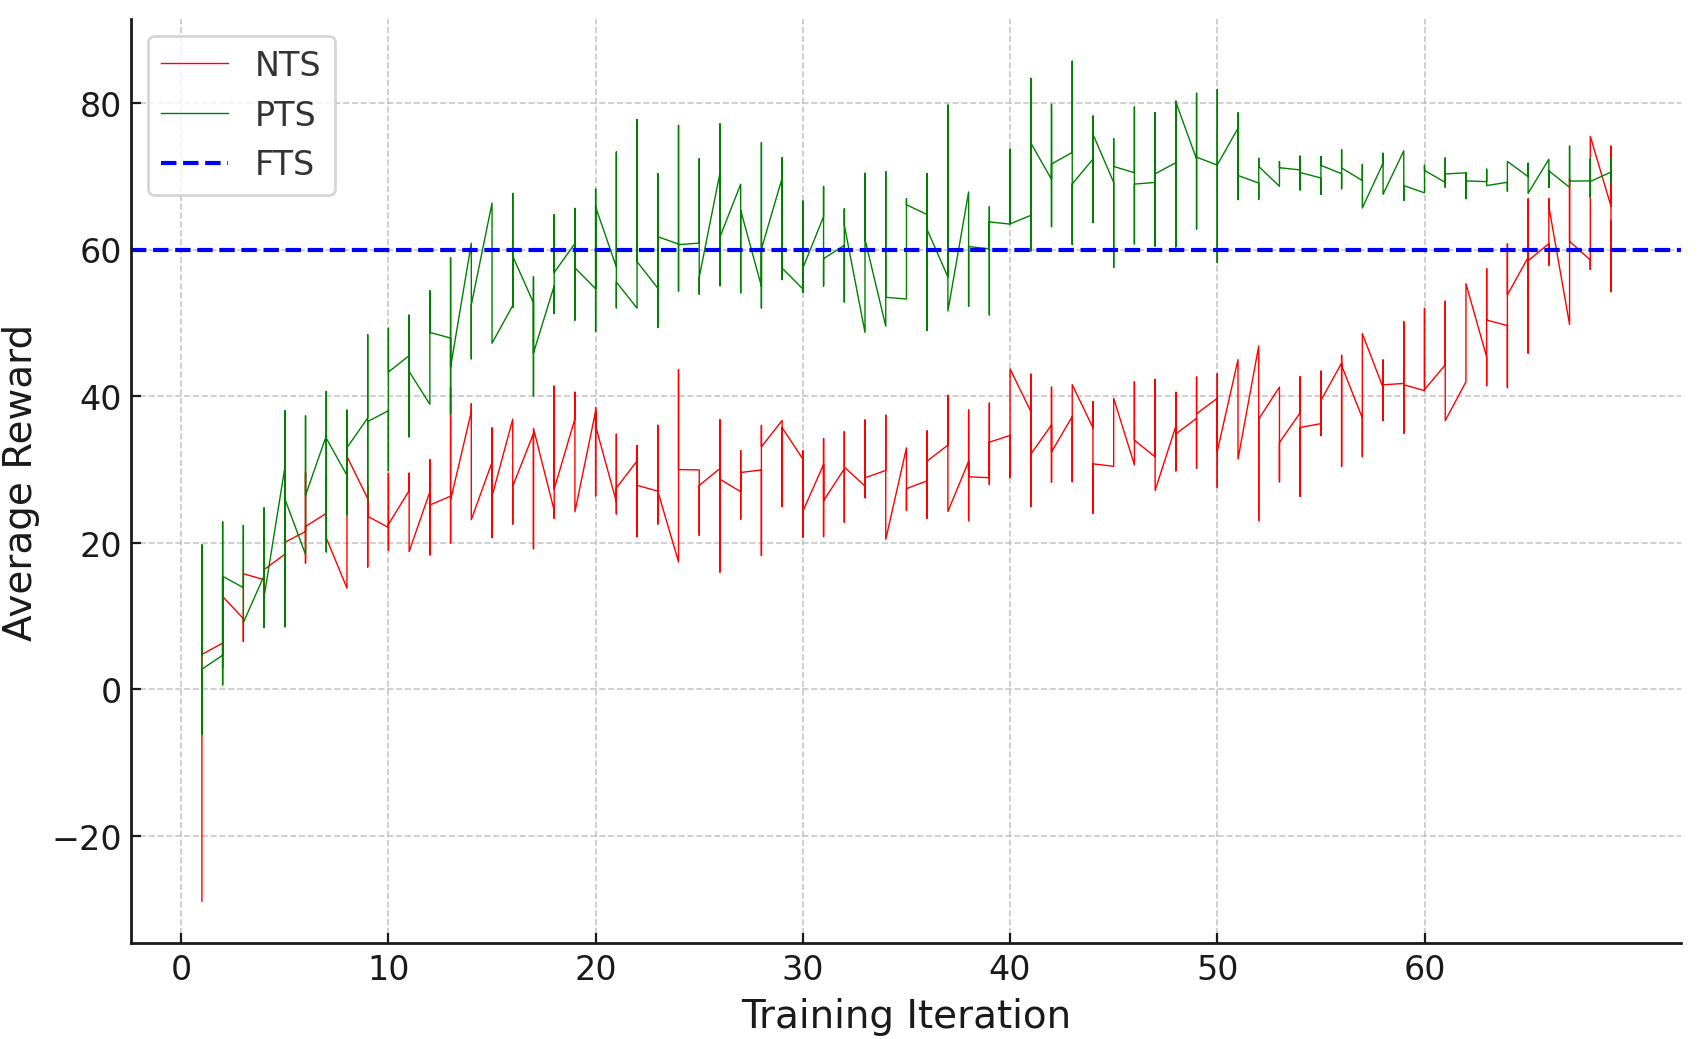
\includegraphics[width=0.9\textwidth]{figures/penalize_learning_curves.png}
  \caption{Learning curves for NTS, PTS, and FTS cases using the \textit{penalize} mode.}
  \label{fig:learning_curves}
\end{figure*}


\begin{table*}[h!]
  \centering
  \caption{Comparison of NTS, PTS, and FTS cases under different modes (correct, penalize, correct\_policy) based on various metrics. \vspace{0.2cm} }\label{tab:results}
  \setlength{\tabcolsep}{5pt}
  \begin{tabular}{cccccccccc}
    \cline{2-10}
                       & \multicolumn{3}{c}{correct} & \multicolumn{3}{c}{penalize} & \multicolumn{3}{c}{correct\_policy}                                                     \\
    \cline{2-10}
                       & NTS                         & PTS                          & FTS                                 & NTS         & PTS & FTS & NTS         & PTS & FTS \\
    \hline
    Scalability        & +                           & +                            & +                                   & ++          & ++  & ++  & +           & +   & +   \\
    Convergence Time   & 62                          & 28                           & 0                                   & 63          & 22  & 0   & 62          & 26  & 0   \\
    Standard Deviation & 2.4                         & 1.5                          & 0.                                  & 2.3         & 2.4 & 0.  & 2.3         & 1.2 & 0.  \\
    Average Reward     & 53                          & 68                           & 60                                  & 52          & 67  & 58  & 53          & 69  & 59  \\
    Constraint Respect & $\emptyset$                 & 1                            & 1                                   & $\emptyset$ & 0.8 & 1   & $\emptyset$ & 1   & 1   \\
  \end{tabular}
\end{table*}
%
%
% The qualitative analysis shows that the \textit{circle\_model} leads to observable circling behaviors around prey, demonstrating the effective impact of organizational specifications on agent behavior. This visually \footnotemark[2] confirms that PRAHOMT can induce desired collective strategies ($\mathbf{C1}$). Additionally, as expected, the \textit{manual\_model} gives good results while being stable.
%
%
%
% Quantitatively, for any mode, the PTS case exhibits faster convergence and higher average rewards compared to the NTS case ($\mathbf{C_3}$), validating the hypothesis that organizational constraints can enhance learning efficiency ($\mathbf{C_2}$). Additionally, we verify the standard deviation to decrease from NTS to PTS and from PTS to FTS $(\mathbf{C_4})$.
%
% The FTS case, serving as a reference, consistently achieves the highest rewards due to pre-defined optimal policies. We also verify the constraint respect to be fully covered in \textit{correct} and \textit{correct\_policy} modes but the \textit{penalize} mode ($\mathbf{C_5}$). Finally, we did not see scalability difficulties when adding up to 30 agents and obstacles for all cases encountered ($\mathbf{C_6}$). From the experiments conducted, the \textit{penalize} mode better faces scalability because it updates its internal policy using optimized computations while \textit{correct} and \textit{correct\_policy} require an aside correction function that may impact the overall computational performance.
%
% The experiments demonstrate that PRAHOMT significantly impacts agent behavior and learning efficiency. The organizational models, especially the \textit{circle\_model}, effectively guide agents towards efficient collective strategies, as evidenced by both qualitative observations and quantitative metrics.
%
The qualitative analysis shows that the \textit{circle\_model} does induce observable circling behaviors around prey, confirming the impact of organizational specifications on agent actions%
\footnote{Screenshots are provided in Annex \ref{sec:screenshots}, as well as a video showing the running \textit{manual\_model} at \url{https://shorturl.at/YRBao}}%
. This visual representation shows alignment with expected collective strategies ($\mathbf{C1}$). The \textit{manual\_model} also exhibited consistent circling behavior, further demonstrating the robustness of predefined policies.

From a quantitative perspective, the metrics provide compelling evidence for the advantages of applying organizational constraints. As illustrated in \autoref{fig:learning_curves}, in the PTS case, agents exhibited faster convergence compared to the NTS case across all modes. This confirms that organizational constraints can accelerate learning ($\mathbf{C2}$). The FTS case, which utilized hand-crafted policies, achieved immediate convergence, as expected, due to the absence of learning.

The average reward metrics reveal that agents guided by the \textit{circle\_model} (PTS) consistently outperformed those in the unconstrained scenario (NTS), achieving higher rewards ($\mathbf{C3}$). This indicates that organizational constraints not only improve learning efficiency but also enhance overall performance. The FTS case, leveraging optimal policies, consistently achieved the highest rewards, highlighting the effectiveness of well-defined constraints. In \autoref{fig:learning_curves}, PTS demonstrates to be even more efficient than the FTS, which was hand-crafted. We also noticed that the \textit{penalize} mode shows slightly better average rewards than \textit{correct} and \textit{correct\_policy} modes. Indeed, \textit{penalize} may authorize not satisfying some organizational specifications if it increases the overall reward.

The standard deviation of rewards, an indicator of performance variability, decreased progressively from NTS to PTS and from PTS to FTS ($\mathbf{C4}$). This reduction in variability suggests that organizational constraints contribute to more stable and consistent agent behavior. As illustrated in \autoref{fig:learning_curves}, PTS shows a lower variance at the end compared to NTS, stabilizing at around 70, probably indicating a stable collective strategy has been found. Again, the \textit{penalize} mode shows a slightly higher deviation because the policy is not strongly constrained by organizational specifications.

Constraint respect, assessed as the adherence to organizational rules, was fully met in the \textit{correct} and \textit{correct\_policy} modes, but not in the \textit{penalize} mode ($\mathbf{C5}$). This demonstrates that while agents can learn to follow constraints effectively, the constraint mode plays a crucial role in their adherence.

Scalability, evaluated by increasing the number of agents and obstacles, was effectively handled in all cases ($\mathbf{C6}$). The \textit{penalize} mode demonstrated superior scalability, as it incorporates optimized computations for policy updates, in contrast to the side correction functions required by the \textit{correct} and \textit{correct\_policy} modes, which can impact computational performance.

In summary, the experimental results show that PRAHOMT enhances both agent behavior and learning efficiency. The \textit{circle\_model} successfully guides agents towards efficient collective strategies, as evidenced by the observed behaviors and quantitative metrics. These findings underscore the utility of organizational constraints in MARL environments and are a first step towards a framework for future research and application.




\section{Conclusion}
This paper introduced PRAHOMT, a novel approach that integrates the MOISE+ organizational model with Multi-Agent Reinforcement Learning (MARL). By constraining the policy space of agents through organizational roles and missions, PRAHOMT improves learning efficiency, safety, and explainability. Our experimental results demonstrate that PRAHOMT outperforms traditional MARL approaches and other optimization techniques in both simple and complex scenarios.

Future work will focus on extending PRAHOMT to handle even more complex organizational structures and dynamic environments, as well as exploring its applicability in real-world systems such as autonomous vehicles and robotic swarms. Additionally, we aim to investigate the scalability of PRAHOMT in large-scale, high-dimensional environments and its integration with other advanced machine learning techniques to further enhance the robustness and adaptability of multi-agent systems.
\label{sec:conclusion}

This paper proposes to see the design of a MAS as a problem under constraint where agents' policies are to be optimized. To integrate the constraints, we proposed the PRAHOMT algorithm to augment the MARL framework with the $\mathcal{M}OISE^+$ model. PRAHOMT constrains agents' training according to organizational specifications. We evaluated PRAHOMT using our proposed proof of concept (PoC) implementation for the \textquote{Simple World Comm} predator-prey environment. Two organizational models were established: a minimally constrained model, \textquote{circle\_model}, and a fully constrained one, \textquote{manual\_model}. We conducted an evaluation of the fully-learned, fine-tuned, or predefined policies based on performance criteria in or after training.
%
The results show that \textquote{circle\_model} provides a relevant tradeoff between constraints and free learning. Despite comprising simple predefined rules, it effectively complements learned behavior.

In addition to constraining agents according to organizational specifications, we also aim to integrate explainability mechanisms. We intend to characterize and curate relevant emergent strategies to include as new organizational constraints in future training. The idea of iterative, mutually beneficial improvement between constrained training and explainability could greatly benefit from hierarchical learning, which helps better characterize and reveal strategies during learning. Furthermore, the initial results obtained with LLM suggest it as a promising complementary tool for PRAHOMT, potentially offering new avenues for explaining collective behavior, especially in scenarios where environments are not visually or intuitively representable.

\begin{acks}
  This work was supported by \emph{Thales Land Air Systems} within the framework of the \emph{Cyb'Air} chair and the \emph{AICA IWG}.
\end{acks}

%%%%%%%%%%%%%%%%%%%%%%%%%%%%%%%%%%%%%%%%%%%%%%%%%%%%%%%%%%%%%%%%%%%%%%%%

%%% The next two lines define, first, the bibliography style to be 
%%% applied, and, second, the bibliography file to be used.

\section*{References}

\bibliographystyle{ACM-Reference-Format}
\renewcommand
\refname{}
\bibliography{references}

\end{document}

%%%%%%%%%%%%%%%%%%%%%%%%%%%%%%%%%%%%%%%%%%%%%%%%%%%%%%%%%%%%%%%%%%%%%%%%